% Define the document style. The thesis stylesheet inherits from 'report'. 
% I had once made a version inheriting from book. However the two versions are almost 
% compatible. The main difference is that the other version supported 'parts'.
% (extended from book) and this does not.
% IST requires the thesis to be written in Arial or similar. Two arguments allow you 
% to define the thesis font: 'Helvetica' and 'AvantGarde', which transforms normal font
% into Helvetica or AvantGarde, respectively... dahhhh!
\documentclass[defaultstyle,10pt,a4paper,master,Helvetica]{thesis}
%\documentclass[defaultstyle,12pt,phd]{thesis}

% Defines an additional alphabet... not required in most cases
% ------------------------------------------------------------
% \DeclareMathAlphabet{\mathpzc}{OT1}{pzc}{m}{it}

% PACKAGE fontenc:
% -----------------
% chooses T1-fonts and allows correct automatic hyphenation.
\usepackage[T1]{fontenc}
\usepackage[latin1]{inputenc}

% PACKAGE babel:
% ---------------
% The 'babel' package may correct some hyphenisation issues of latex. 
% However in most situations it is not required.
\usepackage[portuges]{babel}

% PACKAGE latexsym:
% -----------------
% Defines additional latex symbols. May be required for thesis with many math symbols.
%\usepackage{latexsym}

% PACKAGE amsmath, amsthm, amssymb, amsfonts:
% -------------------------------------------
% This package is typically required. Among many other things it adds the possibility
% to put symbols in bold by using \boldsymbol (not \mathbf); defines additional 
% fonts and symbols; adds the \eqref command for citing equations. I prefer the style
% "(x.xx)" for referering to an equation than to use "equation x.xx".
\usepackage{amsmath, amsthm, amssymb, amsfonts}

% PACKAGE multirow, colortbl, longtable:
% ---------------------------------------
% These packages are most usefull for advanced tables. The first allows to join rows 
% throuhg the command \multirow which works similarly with the command \multicolumn
% The second package allows to color the table (both foreground and background)
% The third package is only required when tables extend beyond the length of one page;
% which typically does not happen and should be avoided
\usepackage{multirow}
\usepackage{colortbl}
% \usepackage{longtable}

% PACKAGE graphics, epsfig, subfigure, caption:
% ---------------------------------------------
% Packages for figures... well you will certainly need these packages, with the exception
% of the 'caption' package. This only allows to define extra caption options.
% Notice that subfigure allows to place figures within figures with its own caption. It
% should be avoided to create an eps file with subfigures. That will mean that you won't be 
% able to reference those subfigures. Instead create an EPS file (the only graphics format supported
% by latex) for each of the subfigures and then use the command \subfigure (see below).
\usepackage{graphicx}
\usepackage{epsfig}
\usepackage[hang,small,bf]{subfigure}
% \usepackage[hang,small,bf]{caption}

% PACKAGE algorithmic, algorithm
% ------------------------------
% These packages are required if you need to describe an algorithm.
% \usepackage{algorithmic}
% \usepackage[chapter]{algorithm}

% PACKAGE natbib/cite
% -------------------
% The two packages are not compatible, and you should use one of the two. Notice however that the
% IEEE BiBTeX stylesheet is imcompatible with the natbib package. If using the IEEE format, use the 
% cite package instead
\usepackage[square,numbers,sort&compress]{natbib}
%\usepackage{cite}

% PACKAGE acronyum
% -----------------
% This package is most usefull for acronyms. The package garantees that all acronyms definitions are 
% given at the first usage. IMPORTANT: do not use acronyms in titles/captions; otherwise the definition 
% will appear on the table of contents.
\usepackage[printonlyused,withpage]{acronym}

% PACKAGE extra_functions
% -----------------
% My Personal package: defines the following commands:
% \fancychapter{chaptername) -> Prints a fancier chapter (you can also use the fancychapter package for this)
% \hline{width} -> use for a replacement of the \hline command
% \Mark1, \Mark2, \Mark3, ...
\usepackage{extra_functions}

% PACKAGE tocloft
% -----------------
% The tocloft package provides means of controlling the typographic design of the Table of Contents,
% List of Figures and List of Tables. New kinds of `List of . . . ' can be defined.
% The package has been tested with the tocbibind, minitoc, ccaption, subfigure, float, fncychap, and hyperref packages.
\usepackage[subfigure]{tocloft}

% PACKAGE babelbib
% -----------------
\usepackage[fixlanguage]{babelbib}
\selectbiblanguage{portuges}

% PACKAGE todonotes
% -----------------
% \usepackage{todonotes}

% PACKAGE IEEEtrantools
% -----------------
% Allows customization of the IEEEtran bibliography style
% \usepackage[retainorgcmds]{IEEEtrantools}

% PACKAGE fixltx2e
% -----------------
% Allows the \textsubscript{} command, among other fixes
\usepackage{fixltx2e}

% PACKAGE longtable
% -----------------
% Use this instead of tabular when you need footnotes inside a table
\usepackage{longtable}

% PACKAGE hyperref
% -----------------
% Set links for references and citations in document
% Some MiKTeX distributions have faulty PDF creators in which case this package will not work correctly
% Long live Linux :D
\usepackage{hyperref}
\hypersetup{ a4paper=true,
             colorlinks=false,
             citecolor=red,
             breaklinks=true,
%            bookmarks=true,		% commented because it generated a warning
             bookmarksnumbered=true,
             bookmarksopen=true,
             pdftitle={T�tulo do PDF},
             pdfauthor={Autor},
             pdfsubject={Tese de Mestrado},
             pdfcreator={LaTeX},
             pdfkeywords={}
}

\def\chapterautorefname{Cap�tulo}
\def\sectionautorefname{Sec��o}
\def\subsectionautorefname{Subsec��o}
\def\figureautorefname{Figura}
\def\tableautorefname{Tabela}

% PACKAGE hypcap
% -----------------
% In case you use the package hyperref to create a PDF, the links to tables or figures
% will point to the caption of the table or figure, which is always below the table or figure itself.
% Therefore the table or figure will not be visible, it is above the pointer and one has
% to scroll up in order to see it.
% If you want the link point to the top of the image you can use this package
\usepackage[all]{hypcap}

% PACKAGE breakurl
% -----------------
% Provides breakable URLs
% This package is designed to be loaded after hyperref to provide a breakable
% hyperlinked \url command under DVI output
%
% Note: apparently not needed when using pdfTeX
% \usepackage{breakurl}

% Set paragraph counter to alphanumeric mode
\renewcommand{\theparagraph}{\Alph{paragraph}~--}

% Page formatting... It was correct for my master thesis... not sure it is still correct
\hoffset 0in
\voffset 0in
\oddsidemargin 0.71cm
\evensidemargin 0.04cm
\marginparsep 0in
\topmargin -0.25cm
\textwidth 15cm
\textheight 23.5cm

\usepackage{fancyhdr}
\pagestyle{fancy}
\renewcommand{\chaptermark}[1]{\markboth{\thechapter.\ #1}{}}
\renewcommand{\sectionmark}[1]{\markright{\thesection\ #1}}
\fancyhf{} \fancyhead[LE]{\bfseries\nouppercase{\leftmark}}
\fancyhead[RO]{\bfseries\nouppercase{\rightmark}}
\fancyfoot[LE,RO]{\bfseries\thepage}
\renewcommand{\headrulewidth}{0.5pt}
\renewcommand{\footrulewidth}{0.5pt}
\addtolength{\headheight}{2pt} % make space for the rule
\fancypagestyle{plain}{%
   \fancyhead{} % get rid of headers
   \renewcommand{\headrulewidth}{0pt} % and the line
   \renewcommand{\footrulewidth}{0pt}
}
\fancypagestyle{blank}{%
   \fancyhf{} % get rid of headers and footers
   \renewcommand{\headrulewidth}{0pt} % and the line
   \renewcommand{\footrulewidth}{0pt}
}
\fancypagestyle{abstract}{%
   \fancyhead{}
   \renewcommand{\headrulewidth}{0pt}
   \renewcommand{\footrulewidth}{0.5pt}
}
\fancypagestyle{document}{%
	\fancyhf{} \fancyhead[LE]{\bfseries\nouppercase{\leftmark}}
	\fancyhead[RO]{\bfseries\nouppercase{\rightmark}}
	\fancyfoot[LE,RO]{\bfseries\thepage}
	\renewcommand{\headrulewidth}{0.5pt}
	\renewcommand{\footrulewidth}{0.5pt}
	\addtolength{\headheight}{2pt} % make space for the rule
}
\setcounter{secnumdepth} {5}
\setcounter{tocdepth} {5}
\renewcommand{\thesubsubsection}{\thesubsection.\Alph{subsubsection}}

\renewcommand{\subfigtopskip}{0.3 cm}
\renewcommand{\subfigbottomskip}{0.2 cm}
\renewcommand{\subfigcapskip}{0.3 cm}
\renewcommand{\subfigcapmargin}{0.2 cm}


% Custom commands for automatic text
% (remember to add {} after each one, or adjacent spaces will be suppressed)
\newcommand{\isocless}{\mbox{ISO/IEC 14443}}
\newcommand{\extlog}{\textit{Extended Logging}}
\newcommand{\emv}{\nameref{sec:ea:emv}}

\newcommand{\acroemph}[1]{\textit{#1}}

\begin{document}

% This solves a pdfTeX warning about page counters related to hyperref
% See: http://en.wikibooks.org/wiki/LaTeX/Packages/Hyperref#Problems_with_Links
\pagenumbering{alph}

% Add PDF bookmark 
\pdfbookmark[0]{Capa}{Titlepage}

%%%%%%%%%%%%%%%%%%%%%%%%%%%%%%%%%%%%%%%%%%%%%%%%%%%%%%%%%%%%%%%%%%%%%%%%%%%%%%%%%%%%%%%%%%%%%%%%
% DEFINE THE TITLEPAGE
% remember that IST requires for the titlepage to be written in portuguese
%%%%%%%%%%%%%%%%%%%%%%%%%%%%%%%%%%%%%%%%%%%%%%%%%%%%%%%%%%%%%%%%%%%%%%%%%%%%%%%%%%%%%%%%%%%%%%%%
% REQUIRED:
% The university logo image: first and second arguments are the (top,left) position of the logo. 
% IST rules force it to be 2cm
\univlogo{3cm}{2cm}{pdf/0_logo_ist_web.pdf}
% OPTIONAL:
% The thesis logo image: first and second arguments are the position of the logo. 
%\thesislogo{2.5cm}{6cm}{img/0_cover_image.png}

% Thesis title
\title{Monitoriza��o Wireless de Pessoas em Ambiente Dom�stico}

% Author and highest current degree (not the one you are applying to)
\author{M�rcio Lu�s Mendon�a de Vasconcelos de N�brega}
\degree{Engenharia Electrot�cnica e de Computadores}
% This is not on the new IST MSc stylesheet... however for PhD dissertations it will most likely be required
% \otherdegree{Mestre}

% The supervisor. Use the second command if required.
% Always remember that 'Professor' should only be used for a supervisor with a Cathedra
\supervisor{Prof. Doutor Renato Jorge Caleira Nunes}
\othersupervisor{Prof. Doutor Ant�nio Manuel Raminhos Cordeiro Grilo}

% Date of the dissertation
\date{Outubro 2012}

% Is this the final version? Place false when delivering the first part.
% The juri members will not be printed in that case. Place true after the juri has accepted the thesis
\finalthesis{true}

% The members of the Juri
% Always remember that 'Professor' should only be used for a juri member with a Cathedra
\presidentofjury{Prof. Doutor Nuno Cavaco Gomes Horta}
\vogalone{Prof. Doutor Carlos Nuno da Cruz Ribeiro}
%\vogaltwo{\_\_\_\_\_\_\_\_\_\_\_\_\_\_\_\_\_\_\_\_\_\_\_\_\_\_\_\_\_\_\_\_\_\_\_\_\_\_\_}
% \vogalthree{Doutor whatever full name 4}
% \vogalfour{Doutor whatever full name 5}
%%%%%%%%%%%%%%%%%%%%%%%%%%%%%%%%%%%%%%%%%%%%%%%%%%%%%%%%%%%%%%%%%%%%%%%%%%%%%%%%%%%%%%%%%%%%%%%%

% print titlepage
\maketitle
\clearpage

% Since I am using double sided pages, the second page should be white.
% Remember that when delivering the dissertation, IST requires for the cover to appear twice.
\thispagestyle{empty}
\cleardoublepage

\setcounter{page}{1} \pagenumbering{roman}

\baselineskip 18pt % line spacing: -12pt for single spacing
                   %               -18pt for 1 1/2 spacing
                   %               -24pt for double spacing

\vspace*{.2\textheight}
\begin{quote}
	\begin{center}
%		\textit{``Some funny/whatever quote, if you want to include one. If not, simply comment this part''} --- Author Name\cite[cap. 5, p. 42]{citacao_anw}
		
		\vspace*{.05\textheight}
		
		\textit{``Uma cita��o engra�ada ou algo do g�nero, se queres incluir uma. Caso n�o, comenta esta parte''}
	\end{center}

\end{quote}

\clearpage

\thispagestyle{empty}
\cleardoublepage

\thispagestyle{plain}
\pdfbookmark{Agradecimentos}{Acknowledgments}
\begin{acknowledgments}
Obrigado ao Pedro Tom�s, o autor original do template para \LaTeX\ (vers�o inglesa).
\end{acknowledgments}

\begin{resumo}
O aumento constante da popula��o idosa mundial tem criado uma enorme quantidade de desafios ao desenvolvimento nacional, � sustentabilidade das fam�lias e � capacidade dos sistemas de sa�de de darem suporte � popula��o idosa. � medida que a tecnologia dos sensores wireless evolui, dispositivos de baixo consumo, reduzida largura de banda e capacidade de armazenamento m�dio, surgem no mercado, com custos de aquisi��o bastante reduzidos. A monitoriza��o de ambientes dom�sticos baseada em sensores wireless, fornece um meio seguro e contido para pessoas idosas, permitindo que estas possam viver nas suas casas o m�ximo tempo poss�vel. Este trabalho introduz o \acf{EMoS}, um sistema desenvolvido no \acf{MiXiM},  onde foi implementado um protocolo de encaminhamento \acf{AODV} e um sistema de localiza��o baseado no HORUS, com a finalidade de monitorizar, num ambiente dom�stico, pessoas idosas ou com necessidades especiais. Os resultados obtidos desta investiga��o demonstram a viabilidade de construir um sistema de monitoriza��o para idosos usando um ambiente simulado onde aspectos de hardware comercialmente dispon�vel foram tamb�m discutidos.
\end{resumo}

\begin{palavraschave}
Redes de Sensores, Pessoas Idosas, Protocolos de Encaminhamento, Localiza��o, MiXiM
\end{palavraschave}

\clearpage
\thispagestyle{empty}
\cleardoublepage

\begin{abstract}
The consistent increase in the world's elder population has been putting a lot of challenges regarding national development, sustainability of families and the ability of health care systems to provide for ageing populations. As wireless sensing technology continues to evolve, devices integrating low-power, low-bandwidth radios and a modest amount of storage, emerge due to considerable reduced costs. Wireless sensors based home monitoring systems provide a safe, sound and secure environment for elder people, enabling them to live in their own home as long as possible. This work introduces the \acf{EMoS}, a \acs{MiXiM} based framework, in which an \acf{AODV} protocol has been implemented together with a modified HORUS system, for tracking and monitoring, in a home environment, elder people or people with special needs. The results obtained from this research demonstrate the feasibility to build a monitoring system for elder care using a simulated environment in which several aspects of the hardware commercially available have been also discussed. 
\end{abstract}


\begin{keywords}
Sensor Networks, Elder Care, Routing Protocols, Indoor Location, MiXiM
\end{keywords}

\clearpage
\thispagestyle{empty}
\cleardoublepage

% This is required for the fancy chapters
\dominitoc
\dominilof
% \dominilot %(I'm not using the List of tables)

%%%%%%%%%%%%%%%%%%%%%%%%%%%%%%%%%%%%%%%%%%%%%%%%%%%%%%%%%%%%%%%%%%%%%%
% List of contents
%\renewcommand{\baselinestretch}{1}
\pdfbookmark[0]{�ndice}{index}
\pdfbookmark[1]{Conte�do}{toc}
\tableofcontents
% \contentsline{chapter}{References}{\pageref{bib}}
\cleardoublepage
%\renewcommand{\baselinestretch}{1.5}

%%%%%%%%%%%%%%%%%%%%%%%%%%%%%%%%%%%%%%%%%%%%%%%%%%%%%%%%%%%%%%%%%%%%%%
% List of figures
\pdfbookmark[1]{Lista de Figuras}{lof}
\listoffigures
\cleardoublepage

%%%%%%%%%%%%%%%%%%%%%%%%%%%%%%%%%%%%%%%%%%%%%%%%%%%%%%%%%%%%%%%%%%%%%%
% List of tables
\pdfbookmark[1]{Lista de Tabelas}{lot}
\listoftables
\cleardoublepage

% %%%%%%%%%%%%%%%%%%%%%%%%%%%%%%%%%%%%%%%%%%%%%%%%%%%%%%%%%%%%%%%%%%%%%%
% % List of algorithms
% Requires packages algorithmic, algorithm
% \pdfbookmark[1]{List of Algorithms}{loa}
% \listofalgorithms
% \cleardoublepage

% %%%%%%%%%%%%%%%%%%%%%%%%%%%%%%%%%%%%%%%%%%%%%%%%%%%%%%%%%%%%%%%%%%%%%%
% % List of acronyms
\pdfbookmark[1]{Lista de Acr�nimos}{loac}

\newcommand{\listacronymsname}{Lista de Acr�nimos}
\newlistof{acronyms}{acr}{\listacronymsname}

\listofacronyms

\begin{acronym}[CDA]
	\acro{BSN}{\acroemph{Body Sensor Network}}
	\acro{BAN}{\acroemph{Body Area Network}}
	\acro{WBAN}{\acroemph{Wireless Body Area Network}}
	\acro{MAC}{\acroemph{Medium Access Control}}
	\acro{GTS}{\acroemph{Guaranteed Time Slots}}
	\acro{WLAN}{\acroemph{Wireless Local Area Network}}
	\acro{WSN}{\acroemph{Wireless Sensor Network}}
	\acro{IR}{\acroemph{Infrared}}
	\acro{CAN}{\acroemph{Car Area Network}}
	\acro{LAN}{\acroemph{Local Area Network}}
	\acro{RFID}{\acroemph{Radio-frequency Identification}}
	\acro{CM}{\acroemph{Case Manager}\acroextra{, profissionais de sa�de do ramo da geriatria.}}
	\acro{ADL}{\acroemph{Activity of Daily Living}}
	\acroplural{ADL}[ADLs]{\acroemph{Activities of Daily Living}}
	\acro{PDA}{\acroemph{Personal Digital Assistant}}
	\acro{BS}{\acroemph{Base Station}}
	\acro{QoS}{\acroemph{Quality of Service}}
	\acro{SPIN}{\acroemph{Sensor Protocolos for Information via Negotiation}}
	\acro{DD}{\acroemph{Direct Diffusion}}
	\acro{AODV}{\acroemph{Ad hoc On-demand Vector Routing}}
	\acro{DSR}{\acroemph{Dynamic Source Routing}}
	\acro{LEACH}{\acroemph{Low-Enegery Adaptive Clustering Hierarchy}}
	\acro{PEGASIS}{\acroemph{Power-Efficient Gathering in Sensor Information Systems}}
	\acro{GEAR}{\acroemph{Geographical and Energy Aware Routing}}
	\acro{TOA}{\acroemph{Time of Arrival}}
	\acro{TDOA}{\acroemph{Time Difference of Arrival}}
	\acro{RSS}{\acroemph{Received Signal Strength}}
	\acro{POA}{\acroemph{Phase of Arrival}}
	\acro{AOA}{\acroemph{Angle of Arrival}}
	\acro{RM}{\acroemph{Radio Map}}
	\acro{RF}{\acroemph{Radio Frequency}\acroextra{, r�dio-frequ�ncia.}}
	\acro{AP}{\acroemph{Access-Point}}
\end{acronym}


\cleardoublepage

% Pages number is starting now with arabic style... until now it was on roman mode
\setcounter{page}{1} \pagenumbering{arabic}
\baselineskip 18pt

% %%%%%%%%%%%%%%%%%%%%%%%%%%%%%%%%%%%%%%%%%%%%%%%%%%%%%%%%%%%%%%%%%%%%%%
% The Introduction:
% %%%%%%%%%%%%%%%%%%%%%%%%%%%%%%%%%%%%%%%%%%%%%%%%%%%%%%%%%%%%%%%%%%%%%%

\fancychapter{Introdu��o}
\label{cap�tulo:introdu��o}
Resumo do cap�tulo.

\section{Motiva��o}
\label{sec��o:introdu��o:motiva��o}
O aumento da esperan�a de vida provoca actualmente um envelhecimento generalizado da popula��o mundial o que coloca diversos desafios ao desenvolvimento nacional, � sustentabilidade das fam�lias e � capacidade dos sistemas de sa�de. Durante anos recentes o n�mero de pessoas no mundo acima dos 60 anos aumentou de 200 milh�es em 1950 para 670 milh�es, sector et�rio que representa j� 20\% da popula��o total nos pa�ses desenvolvidos. \citep{1}. Com a deslocaliza��o das popula��es para os grandes centros, a baixa natalidade, a neglig�ncia familiar, aumenta cada vez mais o n�mero de idosos que vivem sozinhos em suas casas. Esta situa��o cria ansiedade em todos os envolvidos, resultando muitas vezes em internamentos precoces em lares, com um custo elevado e vagas limitadas.

\begin{figure}[!htb]
  \centering
  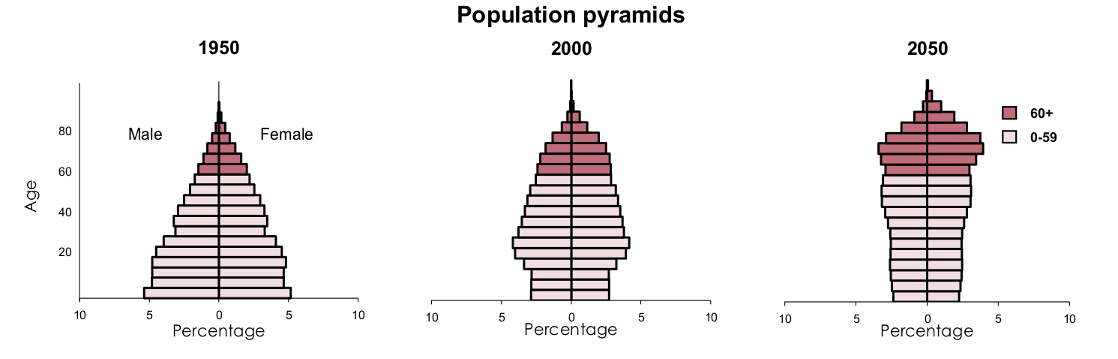
\includegraphics[width=1\textwidth]{img/01_demografia_pt.png}
  \caption{An�lise e previs�o da popula��o em Portugal entre 1950-2050. \cite{1}}
  \label{fig:cap1:demogPT}
\end{figure}

Pessoas com defici�ncias f�sicas ou mentais apresentam tamb�m uma id�ntica necessidade de acompanhamento. Por exemplo, pessoas com defici�ncia mental m�dia, normalmente t�m capacidades sociais e funcionais para serem minimamente independentes, ainda que necessitem de alguma supervis�o e assist�ncia. Normalmente t�m problemas t�o b�sicos como, por exemplo, decidir quando se levantar ou deitar na cama, ou tomar medicamentos � hora certa.

A monitoriza��o de ambos os casos descritos permitiria libertar m�o-de-obra especializada para situa��es de maior depend�ncia, reduzindo custos e aumentando a efici�ncia, notificando m�dicos ou hospitais da mudan�a de sinais vitais que precedam situa��es de risco ou interagindo com ambientes inteligentes.

A evolu��o tecnol�gica dos sensores wireless tem vindo a introduzir no mercado sensores, r�dios e processadores de baixa pot�ncia e baixo custo. Estes dispositivos, com o seu reduzido tamanho, t�m um enorme potencial para o desenvolvimento de aplica��es centradas no utilizador. Com um vasto tipo de sensores, as aplica��es ub�quas\footnote{Aplica��o que tem como objectivo tornar a interac��o entre pessoa e m�quina invis�vel, integrando a inform�tica com ac��es e comportamentos naturais das pessoas.}   podem por isso surgir como alternativa de baixo custo e enorme valor acrescentado para monitoriza��o de pessoas num ambiente dom�stico, criando uma simbiose entre pessoa e m�quina que permita usufruir do direito de viver de forma independente, com privacidade, dignidade e total controlo da pr�pria vida.


\section{Objectivos}
\label{sec��o:introdu��o:objectivos}
Nesta disserta��o � proposto o desenvolvimento de uma solu��o onde uma ou mais pessoas, portadoras de um n� wireless, se movimentam num ambiente onde existem outros n�s wireless. Dever� ser poss�vel localizar cada pessoa e estabelecer uma comunica��o bidireccional entre esta e um servidor central. 

Assim definem-se os seguintes objectivos:
\begin{itemize}
	\item Identificar necessidades num ambiente dom�stico e propor para estas solu��es de hardware existentes no mercado;
	\item Definir a arquitectura do sistema e os papeis de cada interveniente;
	\item Identificar uma plataforma de simula��o existente que permita, de uma forma realista, simular o comportamento do sistema;
	\item Implementar a simula��o de um algoritmo de encaminhamento;
	\item Implementar a simula��o de um algoritmo de localiza��o;
	\item Analisar a simula��o com m�tricas que permitam conhecer o erro de localiza��o, bem como os limites e valores �ptimos do sistema;
\end{itemize}


\section{Principais Contribui��es}
\label{sec��o:introdu��o:contribui��es}
(a escrever no fim)

\section{Organiza��o da Disserta��o}
\label{sec��o:introdu��o:organiza��o}
(a escrever no fim)
%Esta disserta��o encontra-se organizada nos seguintes seis cap�tulos:
%\begin{enumerate}
%	\item \nameref{cap�tulo:introdu��o}
%	\item \nameref{chap:ea}
%	\item \nameref{chap:conclusoes}
%\end{enumerate}
%
%O \autoref{cap�tulo:introdu��o} inclui a introdu��o ao projecto, assim como os seus objectivos, contribui��es do trabalho desenvolvido e a presente explica��o da organiza��o da disserta��o.
%
%O \autoref{chap:ea} ...
%
%Finalmente, no \autoref{chap:conclusoes} s�o tiradas as conclus�es do trabalho efectuado, fazendo-se tamb�m refer�ncias ao trabalho futuro que pode ser feito sobre o apresentado nesta disserta��o.

\cleardoublepage


% %%%%%%%%%%%%%%%%%%%%%%%%%%%%%%%%%%%%%%%%%%%%%%%%%%%%%%%%%%%%%%%%%%%%%%
% Literature Review
% %%%%%%%%%%%%%%%%%%%%%%%%%%%%%%%%%%%%%%%%%%%%%%%%%%%%%%%%%%%%%%%%%%%%%%
\fancychapter{Estado da Arte}
\label{chap:2}

A gera��o actual de casas inteligentes tem tido uma maior evolu��o na intelig�ncia artificial do sistema central, em detrimento dos sistemas de monitoriza��o e controlo. A casa inteligente actual consiste em v�rios electrodom�sticos e outros dispositivos, com sensores, actuadores e/ou monitores biom�dicos, usados pelos residentes numa base di�ria. Em alguns casos a casa � monitorizada recorrendo a tecnologias �udio e v�deo, sendo que estes sistemas apresentam uma excelente forma de monitoriza��o mas t�m algumas desvantagens:

\begin{itemize}
\item Custos elevados devido ao uso de sensores sofisticados e equipamentos �udio-visuais;
\item Custos elevados de instala��o devido � instala��o individualizada;
\item Elevada largura de banda necess�ria;
\item Demasiada intrus�o no quotidiano da pessoa criando um sentimento de falta de privacidade ou desconforto.
\end{itemize}

Tr�s grupos de tecnologias emergem por entre a bibliografia revista:

\begin{itemize}
\item Monitoriza��o com Sinal V�deo ou �udio;
\item Monitoriza��o com Sensores \textit{Wearable};
\item Monitoriza��o com Sensores Dom�sticos.
\end{itemize}

\section{Monitoriza��o com Sinal V�deo ou �udio}
\label{chap:2:sec:1}
Em \cite{2} atrav�s de um sensor wireless equipado com um aceler�metro e transportado pela pessoa, s�o detectadas poss�veis quedas. Por forma a minimizar o n�mero de falsos alarmes, s�o usadas c�maras que cobrem o espa�o, que analisam a posi��o da pessoa e s�o activadas de acordo com a localiza��o do n� m�vel. Essa localiza��o � obtida atrav�s de triangula��o baseada nas posi��es conhecidas dos n�s fixos e a pot�ncia recebida do n� m�vel. � tamb�m apresentada a possibilidade de efectuar transmiss�o de voz utilizando o r�dio IEEE 802.15.4, uma vez que j� existem r�dios com largura de banda necess�ria para efectuar transmiss�o de voz.

\begin{figure}[!htb]
  \centering
  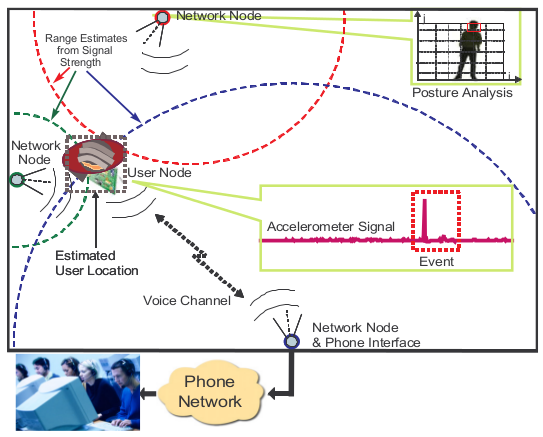
\includegraphics[width=0.65\textwidth]{img/02_video_monit_01.png}
  \caption{Arquitectura do sistema proposto em \cite{2}.}
  \label{fig:1:video_monit_01}
\end{figure}

Em \cite{3} e \cite{4} � feita a combina��o da informa��o fornecida por redes de sensores e sistemas de v�deo-vigil�ncia. Atrav�s de uma infer�ncia l�gica que considera sequ�ncias de eventos s�o tomadas decis�es tal como � poss�vel observar em \ref{fig:2:video_monit_02}. O ocupante da casa usa um sensor n�o intrusivo para determina��o da posi��o e comunica��o por voz, mas n�o � necess�ria qualquer interac��o com a tecnologia. � semelhan�a do trabalho anterior a privacidade � um tema fulcral e todo o tratamento de imagem � feito localmente usando \textit{Smart Cameras} \footnote{c�maras que para al�m de captar imagem tamb�m podem tratar a imagem e obter resultados a partir desta}.

\begin{figure}[!htb]
  \centering
  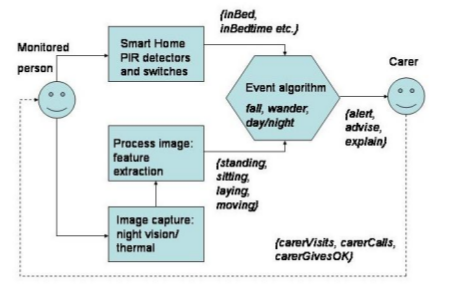
\includegraphics[width=0.75\textwidth]{img/02_video_monit_02.png}
  \caption{Arquitectura de fus�o de decis�o referida em \cite{3}.}
  \label{fig:2:video_monit_02}
\end{figure}

No trabalho \cite{5} � feita a aplica��o de um sistema de monitoriza��o num lar de idosos atrav�s de v�deo e �udio sem recurso a sensores port�teis. O trabalho referencia a insufici�ncia de profissionais em contraste com o r�pido crescimento da popula��o idosa e o pouco tempo que estes t�m dispon�vel para cada idoso. Emerge assim a necessidade de obter um conjunto de dados de forma aut�noma e usado para detectar situa��es de perigo de atempadamente, como por exemplo a instabilidade do andar ou registos comportamentais que favorecem a prescri��o de medicamentos psicotr�picos. Os grandes desafios indicados s�o a localiza��o por v�deo, a correcta identifica��o e marca��o das pessoas no campo de vis�o e a an�lise das suas actividades individuais.

Partindo do conceito \textit{aging in place}, onde idosos vivem de forma independente e segura nas suas pr�prias casas, o trabalho \cite{6} apresenta, a monitoriza��o de quedas mas tamb�m funcionalidades utilit�rias como a detec��o de objectos, calend�rio, v�deo-confer�ncia e livro de endere�os. Recorrendo a c�maras e a t�cnicas de \textit{machine learning} o sistema n�o necessita que o utilizador use um sensor. O sistema tem uma abordagem centralizada devido � forte exig�ncia de processamento em tempo real e mem�ria necess�rias. A detec��o de objectos � feita verificando mudan�as na imagem ou procurando objectos de acordo com as suas caracter�sticas. 

\begin{figure}[!htb]
  \centering
  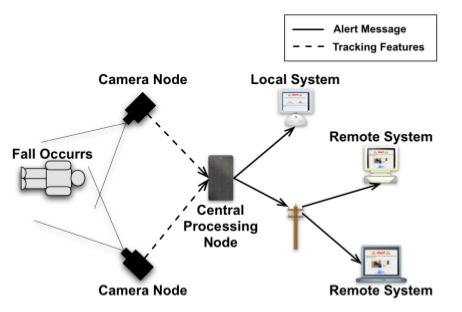
\includegraphics[width=0.8\textwidth]{img/02_video_monit_03.png}
  \caption{Processo de detec��o de quedas e alertas descrito no trabalho \cite{6}.}
  \label{fig:3:video_monit_03}
\end{figure}

Em \cite{7} � utilizado o sinal �udio em conjunto com o v�deo para inferir acerca de uma poss�vel queda. O sinal �udio torna-se essencial para distinguir entre uma pessoa que se sentou ou que caiu. Consideram-se processos de textit{Markov}\footnote{Processo sem mem�ria onde podem ser feitas previs�es do futuro com base somente no estado presente, onde o futuro � independente do passado} que permitem perceber se o comportamento do indiv�duo est� de acordo com o previsto ou n�o e assim tomar as medidas necess�rias.

Embora cada aplica��o tenha as suas mais-valias e a precis�o dos sistemas onde o sinal v�deo � utilizado seja bastante elevada, existe a quest�o da privacidade que resulta numa baixa aceita��o deste tipo de sistemas por parte de pessoas idosas.

A grande preocupa��o nos trabalhos identificados permanece na detec��o de quedas e na fiabilidade dessa detec��o.

\section{Monitoriza��o com Sensores \textit{Wearable}}
\label{chap:2:sec:2}
Com a evolu��o dos sensores wireless aparecem cada vez mais solu��es que permitem fazer uma monitoriza��o cont�nua do estado de sa�de de uma pessoa, independentemente da sua localiza��o ou actividade. A redu��o do tamanho dos sensores permite idealizar a cria��o de vestu�rio com sensores embutidos, suficiente leve e confort�vel para poder ser usado diariamente. Para al�m da monitoriza��o h� tamb�m a possibilidade de administrar medicamentos, recorrendo a actuadores, automaticamente ou de forma manual por um profissional de sa�de de forma remota.

Em \cite{8} � abordada a \acs{BSN}(\textit{Body Sensor Network}) como solu��o para a detec��o precoce de problemas card�acos. Atrav�s de um conjunto de sensores equipados com medidor de temperatura, medidor de pulso, aceler�metro e at� sensores capazes de obter um electrocardiograma\footnote{Representa��o gr�fica da actividade el�ctrica do cora��o} (ECG), um electromiograma\footnote{Representa��o do potencial el�ctrico gerado pelas c�lulas dos m�sculos} (EMG) ou um electroencefalograma\footnote{Representa��o da actividade do c�rebro, obtida por pequenos sinais el�ctricos chamados impulsos} (EEG). O sistema abordado tem um n� coordenador para onde todos os outros enviam informa��o e � usada a norma IEEE 802.15.4, que com suficiente largura de banda permite a transmiss�o da informa��o necess�ria.

\begin{figure}[!htb]
  \centering
  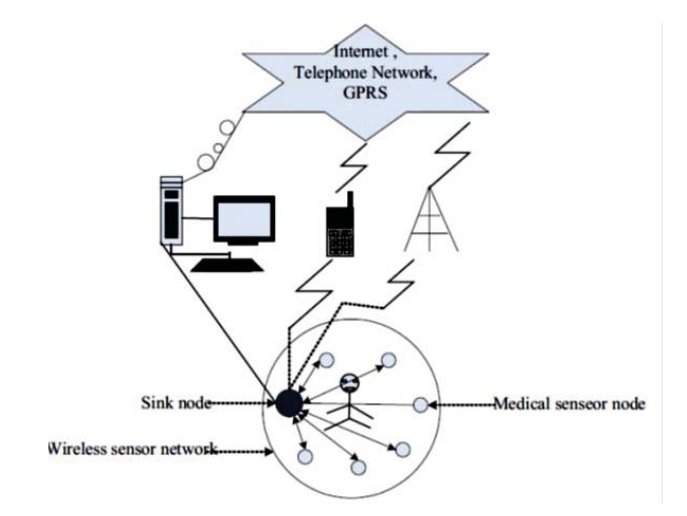
\includegraphics[width=0.5\textwidth]{img/02_body_sensor_network.png}
  \caption{Exemplo de uma \acs{BSN} \cite{8}.}
  \label{fig:4:bsn}
\end{figure}

A aplica��o corre em TinyOS, open-source e com uma gest�o de energia eficiente.
� referida a estrutura modular do sistema operativo que permite escolher componentes conforme a sua aplica��o, o que facilita bastante a utiliza��o de diferentes tipos de sensores. 

De referir o grupo de estudo IEEE 802.15 TG6\footnote{http://www.ieee802.org/15/pub/TG6.html} que pretende estabelecer a norma para as \acs{BAN}s (\textit{Body Area Networks}), que define um protocolo de comunica��o para dispositivos de baixa pot�ncia que operem dentro, em ou � volta do corpo humano.

Em \cite{9} � feita uma discuss�o sobre o tipo de antena e protocolo \acs{MAC} para \acs{WBAN}s, bem como sobre diversas aplica��es para este tipo de redes. Na Figura \ref{fig:5:wban} podemos observar que o tr�fego � categorizado em 3 categorias: \textit{On-demand} iniciado pelo m�dico ou n� coordenador para obter uma determinada informa��o de um ou mais sensores, \textit{Emergency} iniciado pelos n�s quando ultrapassam um determinado \textit{threshold} e \textit{Normal} que n�o apresenta qualquer elemento temporal cr�tico. 

\begin{figure}[!htb]
  \centering
  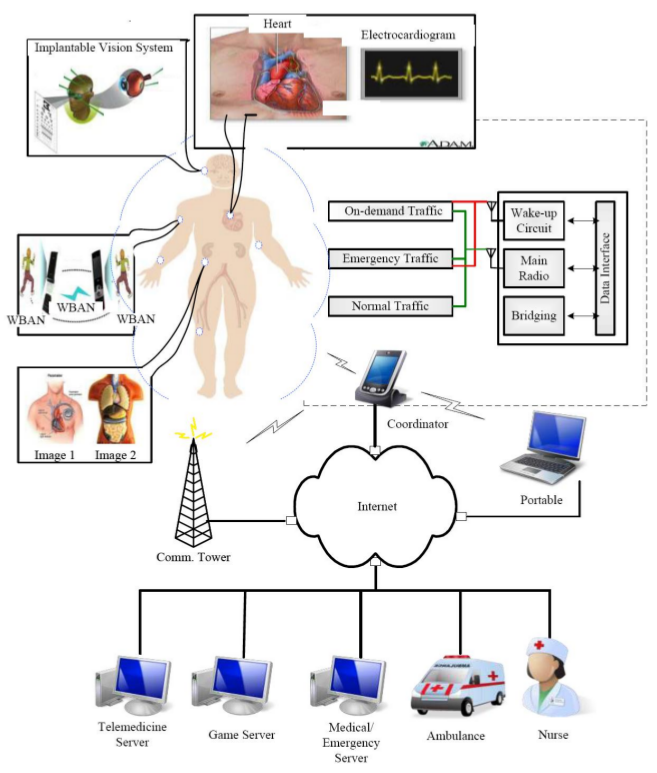
\includegraphics[width=0.80\textwidth]{img/02_wireless_body_area_network.png}
  \caption{Exemplo de uma \acs{WBAN} \cite{9}.}
  \label{fig:5:wban}
\end{figure}

� referido o impacto do corpo na propaga��o do sinal atrav�s da constante diel�ctrica alta que este possui bem como atrav�s da condutividade parcial do tecido muscular que pode absorver parte do sinal, factores que se tornam ainda mais significativos quando as antenas s�o de muito pequena dimens�o. Outro aspecto relevante referido neste trabalho � o facto de n�o existir no IEEE 802.15.4 um mecanismo fi�vel para o envio das mensagens \textit{On-demand} e \textit{Emergency}. Como poss�vel solu��o para este problema � apontada a utiliza��o das IEEE 802.15.4 \acs{GTS}(Guaranteed Time Slots) para lidar com eventos cr�ticos.

Por fim, o trabalho \cite{9} indica atrav�s da Tabela \ref{tab:1:sensor_apps} um conjunto de poss�veis aplica��es para sensores. Doen�as cardiovasculares, detec��o de doen�as oncol�gicas, sistemas de tele-medicina s�o algumas das aplica��es mencionadas.

\begin{table}
	\centering
	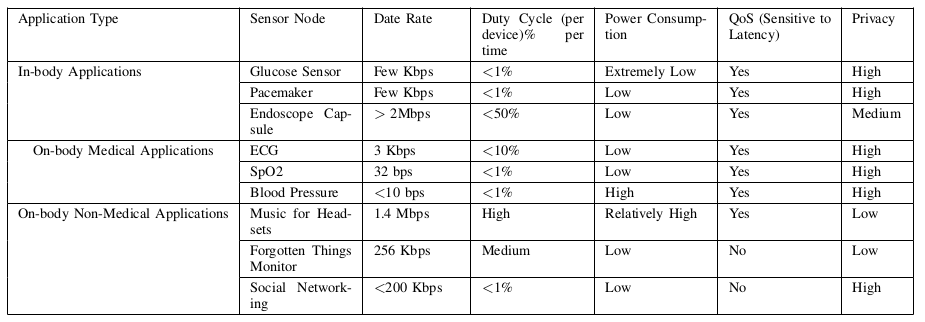
\includegraphics[width=1\textwidth]{img/02_inbody_onbody_applications.png}
  \caption{Aplica��es para redes de sensores \textit{In-body} e \textit{On-body} \cite{9}.}
  \label{tab:1:sensor_apps}
\end{table}

No trabalho \cite{10} � analisada a coexist�ncia entre \acs{WLAN} e \textit{ZigBee} que operam na mesma frequ�ncia de 2.4GHz. A problem�tica de um n�mero elevado de m�dulos \acs{WLAN}, com pot�ncia de transmiss�o mais elevada,  impossibilitar a comunica��o entre m�dulos \textit{ZigBee} � abordada. � sugerida como solu��o a implementa��o de um algoritmo implementado na \acs{WSN} que for�a a que, quando n�o existem frequ�ncias dispon�veis, a \acs{WLAN} seja obrigada a abandonar o canal deixando assim espa�o para o sistema \textit{ZigBee} comunicar. 

\cite{11} prop�e um projecto que integra tecnologias \acs{WSN} com redes p�blicas de comunica��o por forma a construir um sistema eficiente de cuidados de sa�de para idosos em casa. O sistema apresenta quatro funcionalidades principais: monitoriza��o interior, monitoriza��o exterior, actividade e decis�o com base no estado de sa�de. � feita a medi��o e colec��o de par�metros do corpo e da casa e enviada para um servidor central atrav�s de v�rias redes dispon�veis.

Uma das principais desvantagens abordada na pesquisa efectuada � o facto de ter de existir de forma cont�nua um contacto com o corpo do idoso, de v�rios sensores, o que pode causar desconforto. Muitos idosos poder�o n�o estar predispostos para usar uma \acs{BSN} durante um tempo prolongado. Existe tamb�m a possibilidade de interfer�ncia com \textit{pacemakers} ou outros equipamentos m�dicos que tenham sido colocados no idoso.

\section{Monitoriza��o com Sensores Dom�sticos}
\label{chap:2:sec:3}

Neste tipo de monitoriza��o recorre-se a sensores instalados em electrodom�sticos e outros dispositivos utilizados pelos residentes. S�o obtidos padr�es comportamentais atrav�s da correla��o com a utiliza��o dos diversos aparelhos numa casa. Uma das maiores vantagens deste tipo de monitoriza��o � a privacidade, uma vez que a informa��o fornecida por cada sensor n�o cont�m qualquer identifica��o da pessoa que o acciona. Usam-se dispositivos do dia-a-dia o que n�o implica mudan�as de comportamento, como por exemplo com a utiliza��o dos sensores \textit{Wearable} e as \acs{BSN}. Esta abordagem � chamada de \textit{artefact computing model} e representa um paradigma de mudan�a na interac��o pessoa-m�quina na sua forma expl�cita para uma forma impl�cita.

Identificam-se v�rios tipos de sensores aplic�veis a dispositivos dom�sticos:

\begin{itemize}
\item Sensores de press�o;
\item Sensores de movimento e proximidade;
\item Sensores de temperatura;
\item Sensores \acs{RFID};
\item Interruptores;
\item Sensores de vibra��o;
\item Sensores de caudal de �gua ou g�s;
\item Sensores de corrente;
\end{itemize}

No artigo \cite{15} aborda-se a presta��o de cuidados de sa�de aos idosos num complexo constru�do pela \textit{Elite Care}\footnote{http://www. elite-care.com}.Com o objectivo de dar maior autonomia aos residentes s�o criados ambientes personalizados de sensores. O sistema permite identificar residentes que precisam de cuidados imediatos ou iluminar o caminho para um residente que se v� durante a noite � casa-de-banho. A informa��o monitorizada neste sistema pertence a tr�s categorias: sinais vitais, sinais de entrada/sa�da e movimento. Na Tabela \ref{tab:2:pervasiveness}, a partir de um estudo feito com question�rios feitos aos residentes � obtido o grau de intrus�o de cada uma das tecnologias implementadas.

\begin{table}[!htb]
  \centering
  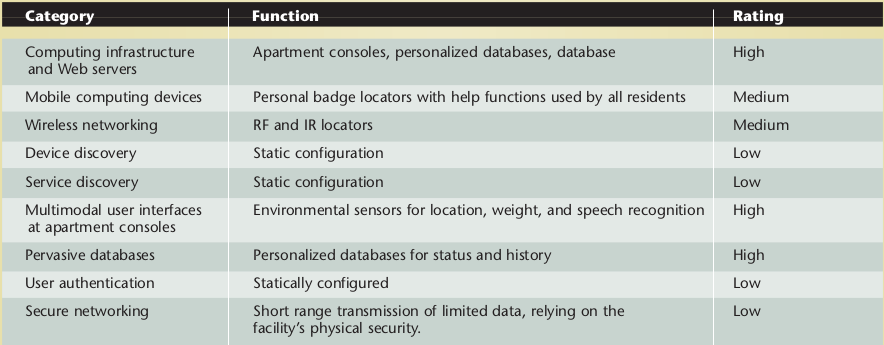
\includegraphics[width=1\textwidth]{img/02_grau_de_intrusao.png}
  \caption{Grau de intrus�o por tecnologia usada em \cite{15}.}
  \label{tab:2:pervasiveness}
\end{table}

\cite{13} usa sensores de press�o para localiza��o. � referida, a t�tulo de exemplo, a aplica��o do sistema a uma pessoa com doen�a de Alzheimer num est�dio m�dio e cuja detec��o do movimento permite activar ecr�s que se ligam quando a pessoa se aproxima e indicam as op��es de percurso na casa. Os melhores sensores conseguem identificar a posi��o e direc��o do utilizador, no entanto a \$10800 por metro quadrado n�o � uma alternativa vi�vel. No projecto s�o usados os \textit{Phidgets} 1.5 polegadas que para 32.5 metros quadrados custa \$4000. Sendo o custo uma desvantagem evidente s�o propostas alternativas, como por exemplo a redu��o de sensores �s zonas previs�veis de passagem ou a utiliza��o de modelos de previs�o que preencham as sec��es sem sensores.

Em \cite{14} � abordado o \textit{PlaceLab}. Situado em Cambrige � um laborat�rio vivo para estudo das tecnologias ub�quas. Est� optimizado para moradias 1 habitantes. Foram criadas para este laborat�rio 15 divis�es e em cada foram colocadas redes de 25 a 30 sensores. 

O projecto \textit{Mediacup} \cite{12} faz uma an�lise da adapta��o de sensores, processamento e comunica��o a dispositivos dom�sticos. Neste artigo uma caneca � adaptada com sensores de movimento e temperatura e ligada em rede com diversos outros dispositivos. Num cen�rio completo, todos os objectos de uso di�rio numa casa poderiam ser adaptados. � usado um processador de 1MHz para redu��o do consumo energ�tico e o carregamento feito usando um campo electromagn�tico instalado num pires. � utilizada a tecnologia \acs{IR} para a comunica��o, atrav�s de mensagens, com transdutores que usam uma arquitectura \acs{CAN}(Car Area Network) integrada por sua vez com uma \acs{LAN} (Figura \ref{fig:6:mediacup})

\begin{figure}[!htb]
  \centering
  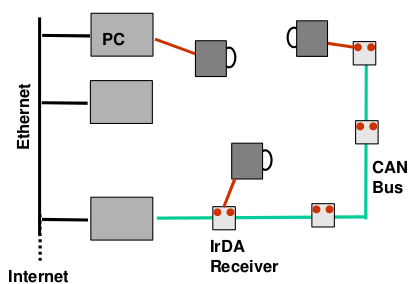
\includegraphics[width=0.75\textwidth]{img/02_mediacup.png}
  \caption{Infraestrutura de rede \textit{Mediacup} \cite{12} que integra \acs{IR}, \acs{CAN} e \acs{LAN}.}
  \label{fig:6:mediacup}
\end{figure}

% Ensure that the next chapter starts in a odd page
\cleardoublepage

% %%%%%%%%%%%%%%%%%%%%%%%%%%%%%%%%%%%%%%%%%%%%%%%%%%%%%%%%%%%%%%%%%%%%%%
% Literature Review
% %%%%%%%%%%%%%%%%%%%%%%%%%%%%%%%%%%%%%%%%%%%%%%%%%%%%%%%%%%%%%%%%%%%%%%
\fancychapter{Trabalho Relacionado}
\label{chap:3}

\section{Monitoriza��o Dom�stica de Idosos}
\label{chap:3:sec:2}
Em \cite{16} faz-se uma an�lise de aspectos fundamentais na monitoriza��o dom�stica de idosos ouvindo os profissionais de cuidados de sa�de. S�o tamb�m neste mesmo trabalho sugeridas diversas propriedades monitoriz�veis e feita uma an�lise global da rede de cuidados de sa�de.

\subsection{Necessidades nos Cuidados de Sa�de}
\label{chap:3:sec:2.1}

No estudo intitulado \textit{``The Activities of Daily Living Study''} em \cite{16} s�o examinados question�rios (91) feitos a profissionais de sa�de que prestam cuidados de monitoriza��o ao domic�lio. Pretende-se determinar a forma como a tecnologia pode ajudar pessoas idosas a envelhecer em casa, tendo em conta os profissionais de sa�de, a necessidade de autonomia do idoso e as necessidades da fam�lia e amigos.

Designam-se \acfp{CM} aos profissionais de sa�de que prestam cuidados ao domic�lio (ex:enfermeiros,m�dicos). Os \acs{CM}s interagem de forma activa com as pessoas idosas presencialmente ou por telefone. Avaliam a habilidade do idoso e a sua predisposi��o para a introdu��o de novos equipamentos. Uma parte significativa da monitoriza��o do \acs{CM} s�o as chamadas \acfp{ADL}, uma lista de actividades que permite medir a fun��o cognitiva e f�sica do idoso (Tabela \ref{tab:1:adls}).

\begin{table}[!htb]
  \centering
  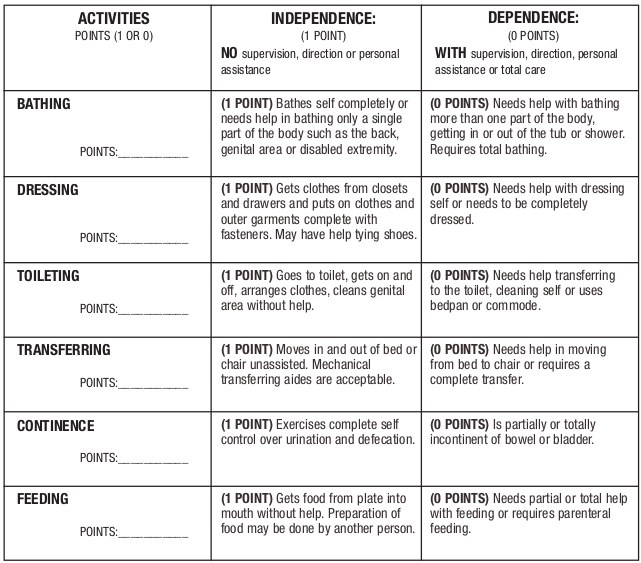
\includegraphics[width=1\textwidth]{img/03_adls.png}
  \caption{�ndice de independ�ncia nas \acs{ADL}s \cite{17}.}
  \label{tab:1:adls}
\end{table}

Esta lista permite definir numa escala de 0-muito dependente a 6-independente, o grau de depend�ncia do idoso. S�o tamb�m apresentados desafios � introdu��o de novas tecnologias pelos \acs{CM}s, nomeadamente:

\begin{itemize}
\item Receio de perda do emprego por parte dos \acs{CM}s;
\item Problemas de aceita��o da nova tecnologia por parte dos idosos, visto que estes t�m tend�ncia a esconder informa��o com receio de irem para a um lar de idosos;
\item Problemas de privacidade;
\end{itemize}

O processo de integra��o de um sistema de monitoriza��o apenas pode ser um sucesso se os profissionais de sa�de estiverem activamente envolvidos na sua implementa��o.

S�o identificadas diversos problemas de sa�de nos idosos, sendo os mais comuns a fraqueza, diabetes, surdez, perda de vis�o, defici�ncia nutricional e dem�ncia moderada.

\begin{table}[!htb]
  \centering
  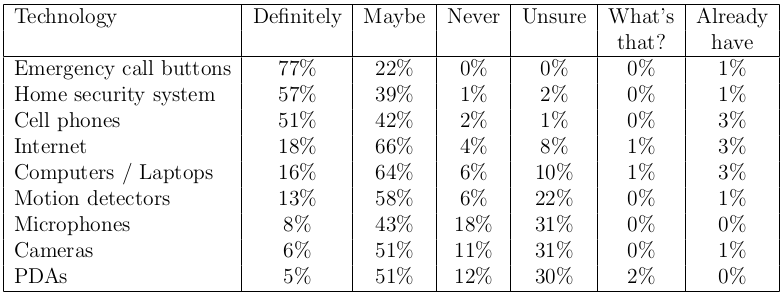
\includegraphics[width=0.95\textwidth]{img/03_elder_tech_acceptance.png}
  \caption{Uso de tecnologia pelos Idosos \cite{16}.}
  \label{tab:3:elderTechAccept}
\end{table}

Na Tabela \ref{tab:3:elderTechAccept} o estudo identifica as tecnologias e a sua aceita��o por parte dos idosos. A comunica��o e a seguran�a s�o identificados claramente como muito valorizados, atrav�s dos bot�es de emerg�ncia e sistemas de seguran�a, enquanto que a tecnologia de monitoriza��o coloca mais incerteza e desconfian�a aos idosos. 

\subsection{Necessidades na Monitoriza��o}
\label{chap:3:sec:2.2}

Com base nos resultados do estudo referenciado na Sec��o \ref{chap:3:sec:2.1} o trabalho \cite{16} faz uma an�lise de diversas tem�ticas de utiliza��o de um sistema de monitoriza��o. 

\textbf{Localiza��o dom�stica}. Determinar se o idoso se levantou pela manh� e os seus padr�es de movimento s�o tamb�m apontadas como duas informa��es importantes. Uma granularidade menor que a divis�o pode por isso ser importante sendo necess�ria uma maior precis�o do sistema. 

\textbf{Agendamento de visitas ao domic�lio}. Saber se o idoso est� ou n�o em casa � apontado pelos \acs{CM}s como um factor de melhoria no agendamento de visitas ao domic�lio.

\textbf{Visitas ao Hospital e Socializa��o}. A integra��o do sistema de monitoriza��o dom�stico com outro baseado em GPS e integrado no sistema de sa�de permitiria para todos os intervenientes no sistema saber onde estava um idoso a qualquer momento para al�m do ambiente dom�stico.

\textbf{N�mero de ocupantes da casa}. Sabendo os padr�es de ocupa��o da casa � poss�vel perceber quais os momentos em que os idosos t�m menos apoio familiar. Em casos mais agudos esta monitoriza��o permitiria determinar se era ou n�o seguro para o idoso continuar em sua casa durante uma determinada altura do dia.

\textbf{Animais de estima��o}. A maioria dos clientes dos \acs{CM}s entrevistados tinham animais de estima��o o que pode ser um problema para sistemas baseados em sensores de press�o.

\textbf{Oportunidades de instrumenta��o}. S�o apresentadas diversas oportunidades de instrumenta��o sem grande necessidade da mudan�a de h�bitos como a aplica��o de sensores a bengalas, andarilhos ou cadeiras de rodas. O facto de existir uma baixa partilha deste tipo de objectos indica que seriam uma boa hip�tese de monitoriza��o n�o-intrusiva. 

\textbf{Privacidade}. � bastante refutada a utiliza��o de c�maras, microfones ou \acs{PDA}s enquanto que os sensores de movimento poderiam ser alternativas vi�veis.

\begin{table}[!htb]
  \centering
  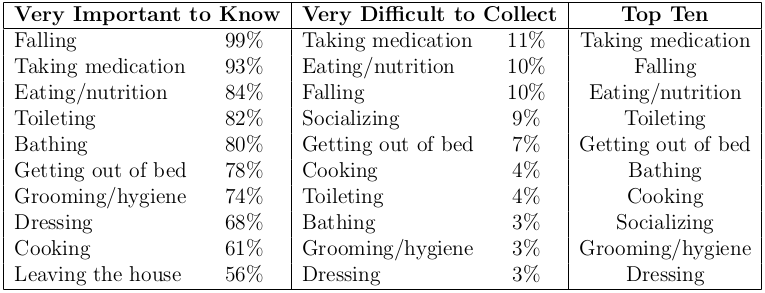
\includegraphics[width=0.9\textwidth]{img/03_adls_monit_rank.png}
  \caption{Classifica��o das \acs{ADL}s por import�ncia, dificuldade em monitorizar e top 10 das mais �teis \cite{16}.}
  \label{tab:4:adlsMonitRank}
\end{table}

\textbf{Escolha das \acs{ADL}s a monitorizar}. Na Tabela \ref{tab:4:adlsMonitRank} � feita uma classifica��o das \acs{ADL}s. O maior valor acrescentado est� naquelas que s�o mais dif�ceis de obter mas mais importantes para serem conhecidas pelo \acs{CM}.

\textbf{Aten��o � actividade das fam�lias ou assistentes}. � importante perceber se existe de facto um apoio real dos familiares ou outros assistentes ao idoso, para al�m de saber que o mesmo est� acompanhado.

\textbf{Monitoriza��o do uso de equipamentos}. A inclus�o nos equipamentos de sa�de de sensores que analisem o estado do equipamento ou a for�a exercida pelo idoso no mesmo, poderiam ajudar a determinar melhor o ponto em que � necess�rio passar de uma bengala para um andarilho ou de um andarilho para uma cadeira de rodas.

\section{Localiza��o em Redes de Sensores Wireless}
\label{chap:3:sec:3}
A chave para obter uma localiza��o fi�vel � representar de forma precisa os efeitos da degrada��o causada pelo canal de propaga��o no sinal. A propaga��o no mundo real sofre diversas perturba��es causadas por obstru��es, reflex�es e pessoas ou objectos em movimento, o que torna esta representa��o um problema de elevada complexidade. Nesta sec��o enumeram-se o tipo de medi��es que permitem inferir uma localiza��o e analisa-se bibliografia relacionada com o objectivo identificar algoritmos de localiza��o distintos, as suas vantagens e desvantagens na aplica��o ao objecto deste trabalho.

\subsection{Medidas de Localiza��o}
\label{chap:3:sec:3.1}
V�rios tipos de medi��es permitem inferir uma localiza��o, nomeadamente:

\begin{itemize}
\item \acs{TOA} (\textit{Time Of Arrival})
\item \acs{TDOA} (\textit{Time Difference Of Arrival})
\item \acs{RSS} (\textit{Received Signal Strength})
\item \acs{POA} (\textit{Phase Of Arrival})
\item \acs{AOA} (\textit{Angle Of Arrival})
\end{itemize}

Na medida do \textbf{\acs{TOA}} mede-se o tempo que um sinal demora a chegar ao n� de destino. A dist�ncia entre origem e destino � obtida multiplicando o atraso entre o momento da transmiss�o e o momento da recep��o do sinal pela velocidade de propaga��o do sinal.O requisito mais importante � a sincroniza��o entre n�s que obriga � exist�ncia de hardware de maior complexidade e a troca de mensagens de sincroniza��o. Ru�do aditivo e efeitos multi-caminho s�o as maiores fontes de erro neste tipo de medi��o.

Utilizando o \textbf{\acs{TDOA}} � medida a diferen�a entre os tempos de chegada em diversos n�s dum mesmo sinal enviado pelo emissor. Um m�nimo de dois n�s � necess�rio para uma estimativa em duas dimens�es da posi��o do do emissor. � semelhan�a do \acs{TOA} � necess�ria sincroniza��o entre os n�s o  que obriga uma vez mais a hardware complexo que aumenta o custo do n�.

O \acs{RSS} � a medida da pot�ncia do sinal recebido. Este m�todo n�o necessita de qualquer hardware especial para sincroniza��o. A pot�ncia do sinal � uma fun��o da dist�ncia, cuja localiza��o pode ser baseada num modelo, onde se admite que as caracter�sticas de propaga��o do sinal s�o bem conhecidas ou ent�o baseada num mapa de medi��es, \acs{RM} (\textit{Radio Map}), onde � feita uma amostragem da pot�ncia em diversas localiza��es.

Com a medida \acs{POA} o objecto de medi��o � o �ngulo de chegada. Este m�todo usa a diferen�a na fase do sinal para determinar a localiza��o do n� emissor.

Por �ltimo a medida de \acs{AOA} indica o �ngulo a que o sinal chega ao receptor, medido com antenas direccionais ou um conjunto de antenas.S�o usadas rela��es geom�tricas simples para calcular a posi��o do n� emissor.

\subsection{Algoritmos de Localiza��o}
\label{chap:3:sec:3.2}
Os esquemas de localiza��o s�o diversos e variam conforme o tipo de aplica��o. 

\begin{figure}[!htb]
  \centering
  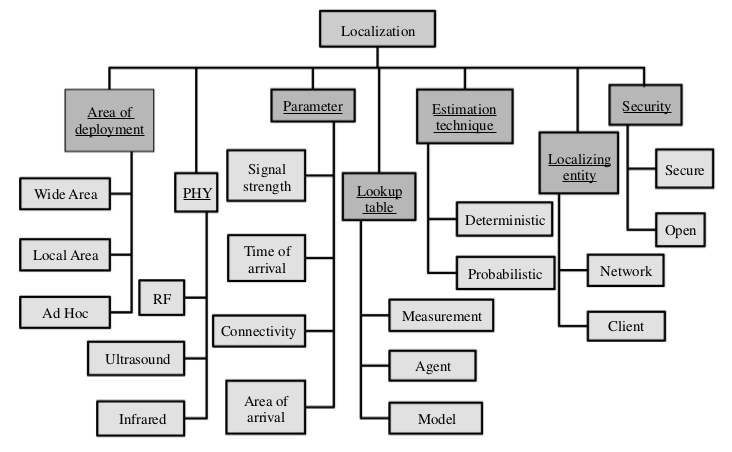
\includegraphics[width=1\textwidth]{img/03_localization_class.png}
  \caption{Classifica��o da localiza��o em redes \acs{WSN} \cite{27}.}
  \label{fig:3:localizationClass}
\end{figure}

A partir da Figura \ref{fig:3:localizationClass} � poss�vel fazer algumas observa��es relativas ao tema deste trabalho que permitir� reduzir a bibliografia a consultar.

\textbf{�rea de Instala��o}: A �rea de instala��o dever� ser local dado uma vez que estamos perante um ambiente dom�stico.

\textbf{PHY}: O meio de transmiss�o do sinal dever� ser a \acs{RF} (R�dio-Frequ�ncia) 

\section{Encaminhamento em Redes de Sensores Wireless}
\label{chap:3:sec:4}
Com a redu��o do custo dos sensores wireless tornou-se poss�vel construir \acs{WSN}s com centenas ou milhares de n�s. A falta de um esquema global de endere�amento, as condicionantes energ�ticas ou a possibilidade de existirem n�s que se movimentam provocando modifica��es na topologia da rede recorrentes, faz surgir a necessidade de encontrar um protocolo de encaminhamento adequado.

\subsection{Desafios e Decis�es de Design}
\label{chap:3:sec:4.1}
Em \cite{18} s�o abordados os diversos desafios no design de protocolos de encaminhamento.

Uma \acs{WSN} apresenta diversas restri��es tais como fornecimento de energia limitado pelo uso de bateria, processamento limitado ou largura de banda reduzida devido a r�dios relativamente simples.

\textbf{Instala��o dos n�s}. A forma como os n�s s�o instalados depende do tipo de aplica��o e pode ser determin�stica ou aleat�ria. Se for aleat�ria a distribui��o n�o � uniforme o que pode requerer \textit{clustering}. A dist�ncia de transmiss�o � reduzida o que obriga a que a comunica��o seja feita atrav�s de v�rios n�s.

\textbf{Toler�ncia a falhas}. Alguns sensores podem falhar devido � falta de energia, dano f�sico ou interfer�ncia. Essas falhas n�o podem por isso condicionar impedir a comunica��o e devem existir protocolos \acs{MAC} e de encaminhamento que consigam detectar essa situa��o e reformular a topologia da rede.

\textbf{Modelo de aquisi��o de dados}. A forma como � feita a aquisi��o de dados � dependente da aplica��o e pode ser orientada ao tempo, para aplica��es de monitoriza��o peri�dica ou ao evento para e � \textit{query}, para n�s que reagem a mudan�as na medi��o de par�metros ou a um pedido feito pela \acs{BS}. 

\textbf{Homogeneidade dos n�s ou liga��es}. Os n�s podem ter todos iguais capacidades sendo a rede homog�nea ou ent�o podem ter capacidades diferenciadas, havendo n�s mais b�sicos e outros mais complexos.

\textbf{Escalabilidade}. Devido ao elevado n�mero de n�s poss�vel numa \acs{WSN} qualquer protocolo de encaminhamento deve ser escal�vel reagindo de forma autom�tica � adi��o ou remo��o de n�s da rede.

\textbf{Din�mica da rede}. A maior parte das arquitecturas assume que os n�s est�o fixos. No entanto para aplica��es em que a topologia muda a estabilidade dos caminhos torna-se um assunto importante e algum tipo de actualiza��o peri�dica ou redescoberta de novos caminhos torna-se necess�rio.

\textbf{Agrega��o de dados}. Os dados de v�rios sensores podem ser agregados para que o n�mero de transmiss�es sofra uma redu��o. A agrega��o pode ser feita com remo��o de duplicados, valores m�nimos, valores m�ximos e valores m�dios. 

\textbf{\acs{QoS}} (\textit{Quality of Service}). Em algumas aplica��es os dados t�m de ser entregues com sucesso ap�s um determinado limite de tempo ap�s a sua obten��o, caso contr�rio perdem significado ou introduzem erros desnecess�rios no sistema. Este limite de tempo pode ser gerido de forma din�mica conforme a qualidade da transmiss�o.

\subsection{Protocolos de Encaminhamento}
\label{chap:3:sec:4.2}
Os protocolos nas \acs{WSN}s podem ser classificados conforme a sua estrutura em \textit{flat-routing} onde todos os n�s t�m as mesmas capacidades e pap�is na rede, \textit{hierarchical-routing} em que existem n�s com capacidades diferenciadas e pap�is diferentes e \textit{location-based routing} onde a posi��o dos n�s � parte integrante do protocolo de encaminhamento.

\title{\textbf{Flat-routing}}

O \acs{SPIN} (\textit{Sensor Protocols for Information via Negotiation}) \cite{20} surge com a necessidade de resolver tr�s problemas nos m�todos cl�ssicos de envio de mensagens (\textit{Flooding} e \textit{Gossiping}), a implos�o causada pela recep��o de v�rias mensagens repetidas vindas de v�rios n�s diferentes, a sobreposi��o resultante da dos dados obtidos por sensores pr�ximos e a falta de adapta��o aos recursos existentes no n�. Na Figura \ref{fig:1:spin} est� um exemplo onde s�o utilizadas os tr�s tipos de mensagens ADV (\textit{advertisment}), REQ (\textit{request} e DATA. O n� A pretende enviar uma mensagem para o n� B e envia um ADV (a). B est� pronto para receber e envia para A um REQ (b). A recebe o REQ e envia uma mensagem DATA para B (c). B continua o processo da mesma forma para os seus n�s vizinhos. Este protocolo permite poupar energia e reduzir o envio de informa��o redundante mas n�o d� garantias de entrega de dados.

\begin{figure}[!htb]
  \centering
  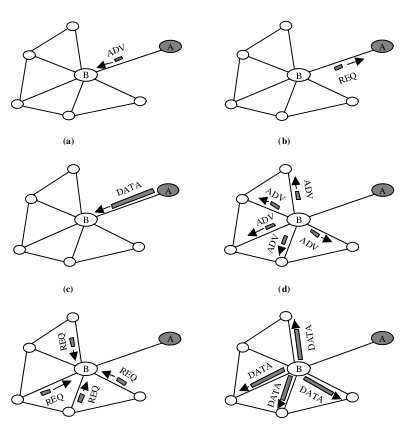
\includegraphics[width=0.85\textwidth]{img/03_spin.png}
  \caption{Protocolo \acs{SPIN} \cite{20}.}
  \label{fig:1:spin}
\end{figure}

O \acs{DD} (\textit{Direct Diffusion}) \cite{21}) introduz um m�todo de procura atrav�s da propaga��o de interesses e cria��o de gradientes constru�dos � medida que um determinado percurso vai sendo utilizado cada vez mais utilizado.

O \acs{AODV} (\textit{Ad hoc On-demand Vector Routing}) \cite{22} introduz o conceito da descoberta de caminhos e da persist�ncia dos mesmos de forma distribu�da por todos os n�s. � um protocolo \textit{On-demand} que s� entra em ac��o quando � necess�rio enviar uma nova mensagem e com mecanismos de \textit{Self-healing} que permitem recuperar um caminho quando por alguma raz�o existiu uma altera��o de topologia. Apresenta duas fases, uma de descoberta de caminho e outra de utiliza��o desse caminho.

Em \cite{23} � abordado o \acs{DSR} (\textit{Dynamic Source Routing}) semelhante ao \acs{AODV} tem como objectivo diminuir a largura de banda consumida pelas mensagens de controlo e necessidade de manuten��o atrav�s de \textit{beacons}. O percurso � guardado na mensagem e vai sendo actualizado � medida que, na fase de descoberta de caminho, esta vai passando em cada n�.

\title{\textbf{Hierarchical-routing}}

No trabalho \cite{24} � proposto o \acs{LEACH} (\textit{Low-Enegery Adaptive Clustering Hierarchy}), um protocolo baseado em \textit{clusters}, que usa coordena��o entre n�s e atrav�s de uma mudan�a aleat�ria do \textit{cluster-head} distribui de forma eficiente o consumo de energia  por todos os n�s. Este protocolo consegue reduzir o consumo de energia at� oito vezes menos que outros protocolos hier�rquicos. O facto dos n�s estarem agrupados em \textit{clusters} permite que a informa��o dos diversos n�s n�o coordenadores possa ser agregada antes de ser enviada para uma \acs{BS}. Como desvantagens tem o facto de n�o ser aplic�vel em redes de grande �rea, tem um \textit{overhead} extra de mensagens controlo e assume que todos os n�s iniciam o seu funcionamento com a mesma energia e que tanto um n� coordenador como um n� simples consumem a mesma energia. Na Figura \ref{fig:2:leach} est� um exemplo de aplica��o.

\begin{figure}[!htb]
  \centering
  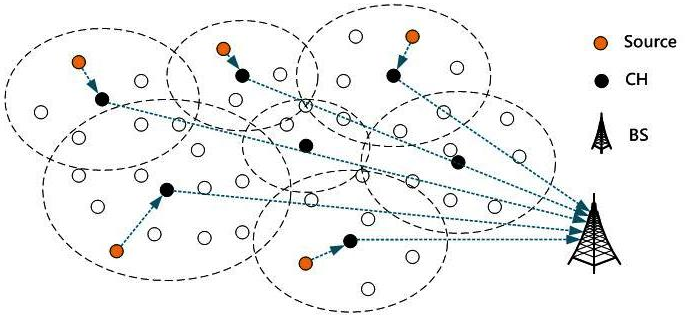
\includegraphics[width=1\textwidth]{img/03_leach.png}
  \caption{Exemplo de funcionamento do protocolo \acs{LEACH}.}
  \label{fig:2:leach}
\end{figure}

Outro protocolo hier�rquico � o \acs{PEGASIS} (\textit{Power-Efficient Gathering in Sensor Information Systems}) \cite{25} que surge como um melhoramento do \acs{LEACH}. Este protocolo aumenta o tempo de vida de cada n� usando t�cnicas colaborativas, onde cada n� fala apenas com o seu vizinho mais pr�ximo e transmite alternadamente para a \acs{BS}, eliminando assim a necessidade de forma��o de \textit{clusters} de forma din�mica e exist�ncia de v�rios n�s coordenadores. Como desvantagens o facto de se assumir que todos os n�s conseguem comunicar com a \acs{BS} directamente, que os n�s t�m o mesmo n�vel de energia e podem desligar-se ao mesmo tempo ou a possibilidade do coordenador �nico se tornar um \textit{bottleneck} no sistema.

\title{\textbf{Geographic-based Routing}}

Em \cite{26} � abordado o \acs{GEAR} (\textit{Geographical and Energy Aware Routing}). Este protocolo surge em redes com um n�mero elevado de sensores e onde poder�o ser feitas consultas a determinadas zonas geogr�ficas da rede, sem que tal seja feito com recurso a \textit{flooding}. S�o utilizadas heur�sticas baseadas na energia dos n�s e informa��o sobre a sua posi��o para encaminhar um pacote para uma determinar regi�o.

% Ensure that the next chapter starts in a odd page
\cleardoublepage

% %%%%%%%%%%%%%%%%%%%%%%%%%%%%%%%%%%%%%%%%%%%%%%%%%%%%%%%%%%%%%%%%%%%%%%
% State of the art
% %%%%%%%%%%%%%%%%%%%%%%%%%%%%%%%%%%%%%%%%%%%%%%%%%%%%%%%%%%%%%%%%%%%%%%

\fancychapter{Ambiente de Trabalho}
\label{chap:4}
As \acsp{WSN} s�o compostas por in�meros sensores wireless munidos de reduzidas capacidades de processamento, comunica��o e armazenamento. Antes da implementa��o de aplica��es que recorram a sensores wireless e respectiva arquitectura base (por exemplo, o TinyOS \cite{32}) em aplica��es reais, torna-se necess�rio avaliar a efici�ncia e robustez das mesmas, recorrendo a simula��es que englobem tanto a componente aplicacional do n� como a rede no seu todo. 

Nesta disserta��o sugere-se a cria��o de um ambiente de trabalho que resulta da utiliza��o conjunta de tr�s sistemas: a \acf{OMNeT++} \cite{33}, uma \textit{framework} base de simula��o por m�dulos,  o \acf{MiXiM} \cite{34}, uma uni�o de v�rias \textit{frameworks} para \acs{OMNeT++}, vocacionadas para a simula��o de sensores wireless e um componente de simula��o de obst�culos para o MiXiM \cite{35}.

\begin{figure}[!htb]
  \centering
  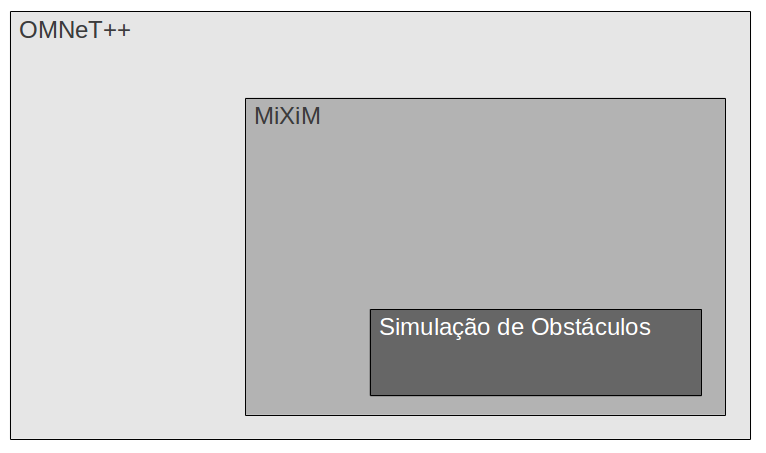
\includegraphics[width=0.70\textwidth]{img/04_framework_overview.png}
  \caption{Representa��o modular do ambiente de trabalho.}
  \label{fig:1:frameworkOverview}
\end{figure}

\section{Objective Modular network Test-bed (OMNeT++)}
\label{chap:4:sec:1}
O \acs{OMNeT++}\footnote{http://http://www.omnetpp.org/} � uma plataforma de simula��o baseada em m�dulos, escrita em C++ e com um IDE baseado em Eclipse. 

O \acs{OMNeT++} foi a plataforma base escolhida para este trabalho pelas seguintes raz�es:

\begin{itemize}
\item A partilha dos resultados deste trabalho com a comunidade \acs{OMNeT++}, promovendo a continuidade do trabalho efectuado nesta disserta��o;
\item A reutiliza��o e combina��o de m�dulos j� constru�dos;
\item A orienta��o por objectos que permite uma flex�vel extens�o das classes base;
\item A exist�ncia de um ambiente gr�fico autom�tico para uma melhor visualiza��o e \textit{debug} da simula��o;
\item A biblioteca extensa inclu�da que oferece suporte para estat�stica, colec��o de dados, apresenta��o gr�fica, n�meros aleat�rios e estruturas de dados;
\item A possibilidade simular v�rios cen�rios mudando apenas par�metros num ficheiro de configura��o, sem necessidade de nova compila��o.
\end{itemize}

Cada m�dulo pode ser do tipo simples ou composto. Os m�dulos compostos s�o constitu�dos por m�dulos simples ou por outros m�dulos compostos criando assim uma estrutura hier�rquica de depend�ncia.Todos os m�dulos assentam sobre um m�dulo de sistema, respons�vel pela realiza��o da simula��o. A comunica��o entre m�dulos � feita atrav�s do envio de mensagens, que podem ser t�o especializadas quanto o necess�rio, enviadas por canais de comunica��o de entrada e sa�da. Na Figura \ref{fig:2:omnet} est� um diagrama exemplificativo desta arquitectura.

\begin{figure}[!htb]
  \centering
  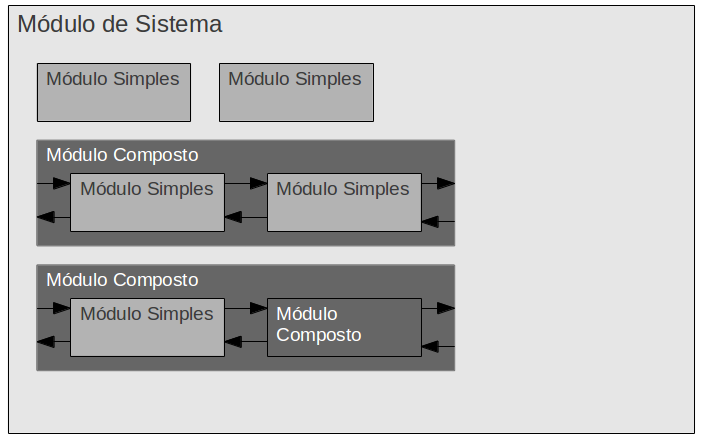
\includegraphics[width=0.80\textwidth]{img/04_omnet.png}
  \caption{Estrutura modular do OMNeT++.}
  \label{fig:2:omnet}
\end{figure}

A topologia de cada m�dulo e a forma como interliga com outros, � descrita utilizando a linguagem \acf{NED} sendo posteriormente a implementa��o feita em C++. � um utilizado um ficheiro de configura��o (ex: omnetpp.ini) que permite criar diversos cen�rios poss�veis definindo para cada um, por exemplo, par�metros dos m�dulos, tempo de simula��o, \textit{seed} para n�meros aleat�rios, etc. Esta solu��o permite a utiliza��o de apenas um execut�vel para diversas cen�rios.

Na Figura \ref{fig:3:omnetInternal} � poss�vel observar a estrutura interna de um execut�vel \acs{OMNeT++}.

\begin{figure}[!htb]
  \centering
  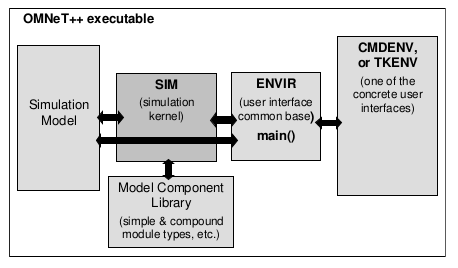
\includegraphics[width=0.85\textwidth]{img/04_omnet_internal.png}
  \caption{Arquitectura l�gica de um execut�vel OMNeT++ \cite{33}.}
  \label{fig:3:omnetInternal}
\end{figure}

A \textit{Model Component Library} cont�m o c�digo compilado dos m�dulos simples e compostos. Os m�dulos s�o instanciados e o \textit{Simulation Model} � constru�do pelo \textit{Simulation Kernel} (SIM) no in�cio da execu��o. A simula��o � ent�o executada num ambiente definido pelo utilizador que pode ser um dos disponibilizados no \acs{OMNeT++} (\textit{Tkenv} ou \textit{Cmdenv}) ou outro (ambiente criado pelo utilizador ou embebido noutra aplica��o). Para cada ambiente podem escolhidos ficheiros de configura��o (*.ini) e cen�rios definidos em cada ficheiro de configura��o. O ambiente \textit{Cmdenv} corre na linha de comandos de forma r�pida enquanto que o ambiente \textit{Tkenv} fornece um ambiente gr�fico capaz de animar de forma autom�tica o percurso das mensagens ou as posi��es dos n�s (Figura \ref{fig:4:omnetTkenv}).

\begin{figure}[!htb]
  \centering
  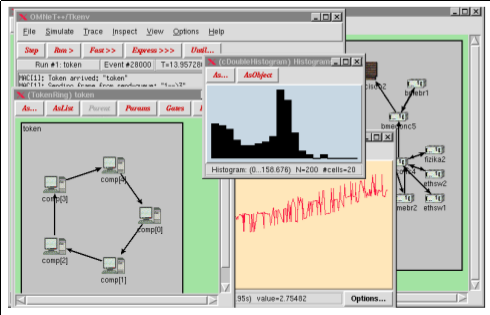
\includegraphics[width=1\textwidth]{img/04_omnet_tkenv.png}
  \caption{Ambiente de simula��o Tkenv no OMNeT++ \cite{33}.}
  \label{fig:4:omnetTkenv}
\end{figure}

\section{Mixed Simulator (MiXiM) para OMNeT++}
\label{chap:4:sec:2}
O \acs{MiXiM}\footnote{http://mixim.sourceforge.net/} resulta da combina��o de quatro \textit{frameworks}: a \acf{MF} que introduz suporte � mobilidade, o \acf{ChSim} que adiciona modelos detalhados de propaga��o, o MAC Simulator e a Positif Framework que adicionam o \acs{MAC}. Esta plataforma foi criada especificamente para simula��o de redes wireless introduzindo v�rias novidades �teis na simula��o de \acsp{WSN}, tais como:

\begin{itemize}
\item M�dulos para sensores wireless com diversas camadas e simula��o de bateria;
\item \acsp{NIC} de sensores wireless existentes no mercado (Texas Instruments CC1100 e CC2420);
\item Novos modelos de propaga��o de sinal, como por exemplo o \textit{Two-Ray Ground Path Loss} ou o \textit{Log-normal Shadowing};
\item A possibilidade de ter na mesma simula��o v�rios canais para diferentes frequ�ncias o que permite ter na mesma simula��o comunica��o WI-FI e \acs{GSM}.
\item A decis�o da qualidade do sinal e sua recep��o feita pelo n� receptor;
\item Novos m�dulos de mobilidade.
\end{itemize}

\begin{figure}[!htb]
  \centering
  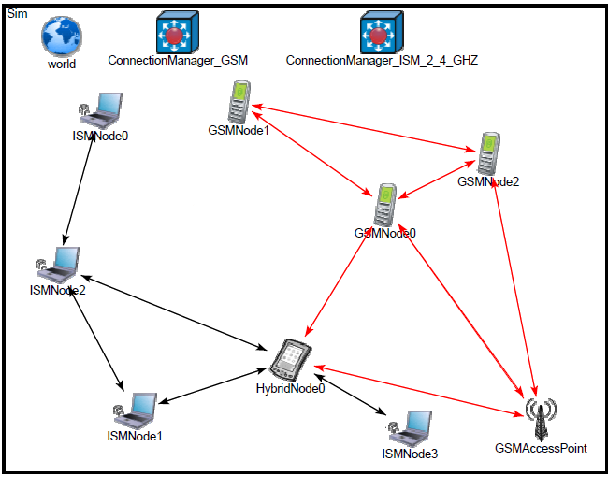
\includegraphics[width=0.85\textwidth]{img/04_mixim.png}
  \caption{Simula��o de uma rede no MiXiM \cite{34}.}
  \label{fig:5:mixim}
\end{figure}

Na Figura \ref{fig:5:mixim} temos a estrutura do \acs{MiXiM} que pode ser dividido em dois tipos de m�dulos:

\begin{itemize}
\item M�dulos de Simula��o: m�dulo \textit{world} respons�vel pela configura��o do ambiente (dimens�es da �rea de trabalho, gest�o de par�metros globais) e \textit{ConnectionManager} respons�vel pela gest�o das liga��es entre n�s. De notar que o MiXiM suporte v�rios n�s de liga��o, tantos como os canais de transmiss�o existentes;
\item M�dulos de N�: m�dulos com v�rios sub-m�dulos que implementam cada uma das camadas l�gicas e f�sicas presentes num n� de uma rede wireless.
\end{itemize}

\begin{figure}[!htb]
  \centering
  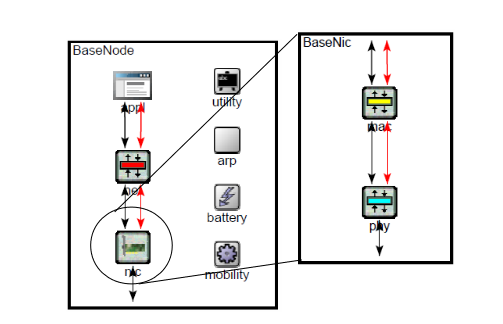
\includegraphics[width=0.70\textwidth]{img/04_mixim_node_module.png}
  \caption{M�dulo de n� no MiXiM \cite{34}.}
  \label{fig:6:miximNode}
\end{figure}

\begin{figure}[!htb]
  \centering
  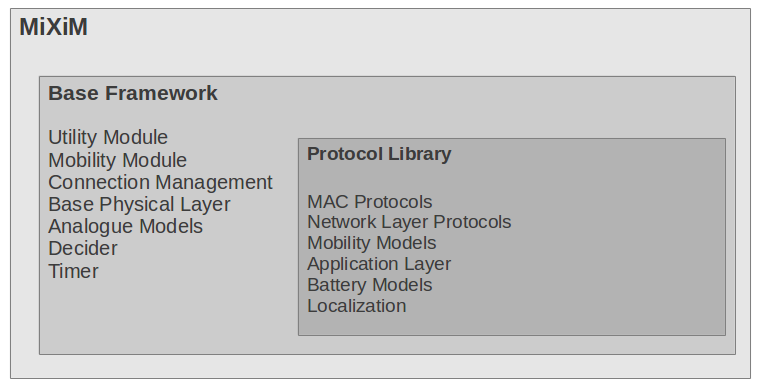
\includegraphics[width=0.85\textwidth]{img/04_mixim_logic_layers.png}
  \caption{Divis�o l�gica da \textit{framework} MiXiM.}
  \label{fig:7:miximLogicLayers}
\end{figure}

Na Figura \ref{fig:6:miximNode} observa-se em detalhe o m�dulo de n� onde est�o presentes as camadas l�gicas de um sensor wireless, o \acs{NIC} constitu�do pelas \acs{PHY} e \acs{MAC}, a camada \textit{Network} (Netw) e a camada de aplica��o. Existem ainda paralelamente v�rios sub-m�dulos, nomeadamente o \textit{mobility} que trata da posi��o e movimenta��o do n� na �rea de trabalho, o \textit{battery} que simula o consumo de energia, o \textit{arp} que trata do endere�amento e o \textit{utility} que serve para efeitos utilit�rios na partilha de informa��o durante a simula��o.

O \acs{MiXiM} pode ser dividido de forma l�gica numa plataforma base e numa biblioteca de protocolos conforme se pode observar na Figura \ref{fig:7:miximLogicLayers}. A plataforma base tem todos componentes necess�rios para criar uma simula��o. A biblioteca de protocolos tem diversas extens�es da plataforma base que permitem diversificar a quantidade de protocolos e modelos existente.

Importa analisar como funciona a camada \acs{PHY} no \acs{MiXiM}. A pot�ncia do sinal � influenciada pelo canal de propaga��o, influ�ncia que pode ser modelada por atenua��es causadas por efeitos de \textit{path loss}\footnote{Atenua��o causada pelo ar.}, \textit{shadowing}\footnote{Atenua��o causada por obst�culos.} e \textit{fading}\footnote{Atenua��o causada pela multi-propaga��o de um sinal derivada de diversas reflex�es.}. Para al�m disso tamb�m a frequ�ncia do sinal, a pot�ncia de envio e o \textit{bit-rate} (modula��o e codifica��o) no tempo, espa�o e frequ�ncia podem afectar a pot�ncia do sinal recebido.

Para modelar este complexo processo o MiXiM implementa uma classe especial de sinal que � associada a cada mensagem e implementa a camada \acs{PHY} tal como esquematizado na Figura \ref{fig:8:miximPhy}.

\begin{figure}[!htb]
  \centering
  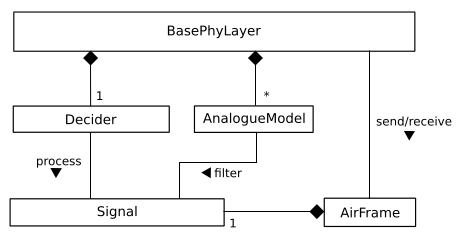
\includegraphics[width=0.75\textwidth]{img/04_mixim_phy.png}
  \caption{Camada PHY do MiXiM \cite{34}.}
  \label{fig:8:miximPhy}
\end{figure}

Quando recebe uma mensagem vinda do exterior (\textit{AirFrame}), a camada \acs{PHY} envia a mensagem para o modelo anal�gico que ir� calcular a atenua��o do sinal e para o \textit{Decider} que verifica se o sinal � ru�do com base na pot�ncia recebida e calcula os bit-errors. Depois deste momento a camada \acs{PHY} calcula o atraso de propaga��o e de transmiss�o da mensagem cabendo � camada \acs{MAC} determinar com base nos \textit{bit errors} se mensagem � v�lida ou n�o.


\section{Simula��o de Obst�culos para MiXiM}
\label{chap:4:sec:3}
Embora esteja referida em \cite{34}, a simula��o de obst�culos, como parte integrante do MiXiM, esta nunca chegou a ser implementada. Assim foi necess�rio procurar uma solu��o que permitisse simular a exist�ncia de obst�culos no ambiente de trabalho.

O trabalho \cite{35} implementa a simula��o de obst�culos no MiXiM e a sua representa��o no ambiente Tkenv. O modelo descrito n�o contempla efeitos de reflex�o ou difrac��o e pretende ser computacionalmente r�pido. A configura��o dos obst�culos � feita atrav�s de um ficheiro XML. Na \lstlistingname{} \ref{list:1:obstaclesXML} est� o c�digo XML necess�rio para desenhar o obst�culo da Figura \ref{fig:9:miximWithObstacles}.

\begin{workflow-code}{Exemplo de configura��o XML de obst�culos.}{list:1:obstaclesXML}
<obstacles>
   <poly id="wall#0" type="brickWall20cm" color="#F00" shape="12.8,10 13,10 13,15 12.8,15" />
</obstacles>
\end{workflow-code}

\begin{figure}[!htb]
  \centering
  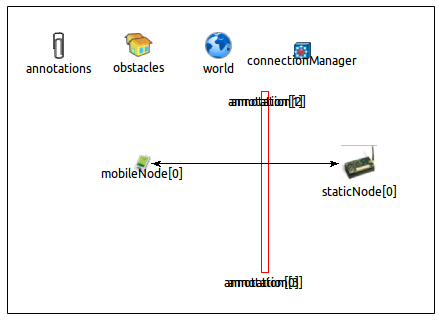
\includegraphics[width=0.75\textwidth]{img/04_mixim_with_obstacles.png}
  \caption{Simula��o de uma rede MiXiM com obst�culos.}
  \label{fig:9:miximWithObstacles}
\end{figure}


Para melhor perceber a solu��o encontrada analisa-se a base matem�tica do modelo.

Sabendo que a pot�ncia recebida de um sinal � dada por:

\begin{equation}
	P_r[dBm] = P_t[dBm] + G_t[dB] + G_r[dB] - \sum{L_x[dB]}
\end{equation}

onde \begin{math}P\end{math} � pot�ncia, \begin{math}G\end{math} � ganho e \begin{math}L_x\end{math} s�o os termos que traduzem as perdas. No MiXiM as perdas j� s�o calculadas como descrito na sec��o anterior pela camada \acs{PHY} mas n�o contemplam as perdas provocadas por obst�culos. 

� ent�o sugerido um termo para a pot�ncia provocada por obst�culos:

\begin{equation}
	L_{obs}[dB] = \beta{n} + \gamma{d_m}
\end{equation}

Os termos \begin{math}\beta{}\end{math} e \begin{math}\gamma{}\end{math} s�o calculados com base nos resultados obtidos experimentalmente e representam a atenua��o por metro e a atenua��o por parede respectivamente. Para o trabalho \cite{35} os valores obtidos foram \begin{math}\beta{}\approx{9dB}\end{math} e \begin{math}\gamma{}\approx{0.4dB/m}\end{math}. 

Devido � n�o utiliza��o de n�s reais neste trabalho, que permitissem chegar a valores reais, optou-se por considerar, com base no Tabela \ref{tab:1:attenuationPerInch} do manual da \textit{3Com Wireless Antenas}\footnote{http://www.scribd.com/doc/32613170/3Com\%C2\%AE-Wireless-Antennas}, os seguintes valores:

\begin{table}[!htb]
	\centering
\begin{tabular}{ |c|c|c|}
	\hline
  	Profundidade(cm) & \begin{math}\beta{}\end{math}(dBm)  & \begin{math}\gamma{}\end{math}(m)\\
  	\hline
  	20 & 106.3 & 0 \\
  	10 & 26.575 & 0 \\
  	\hline
\end{tabular}
	\caption{Valores de atenua��o por metro e por parede usados neste trabalho.}
	\label{tab:1:attenuationValues}
\end{table}

\begin{table}[!htb]
  \centering
  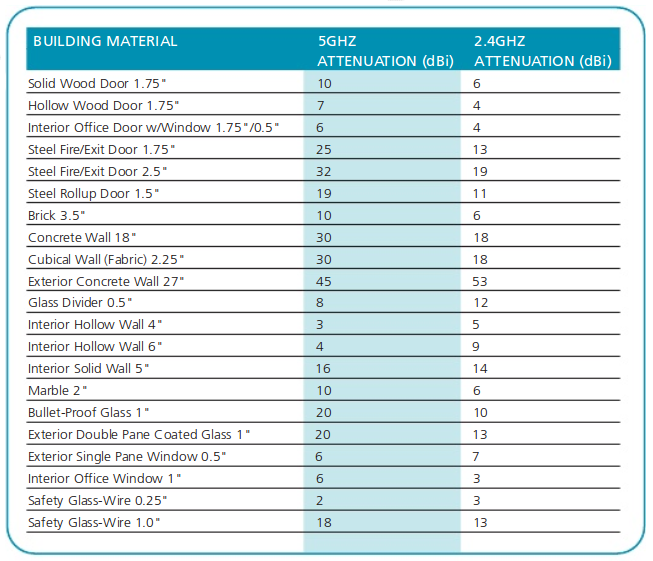
\includegraphics[width=1\textwidth]{img/04_attenuation_per_inch.png}
  \caption{Atenua��o de materiais de constru��o comuns para frequ�ncias de 5GHz e 2.4 GHz.}
  \label{tab:1:attenuationPerInch}
\end{table}




% Ensure that the next chapter starts in a odd page
\cleardoublepage

% %%%%%%%%%%%%%%%%%%%%%%%%%%%%%%%%%%%%%%%%%%%%%%%%%%%%%%%%%%%%%%%%%%%%%%
% State of the art
% %%%%%%%%%%%%%%%%%%%%%%%%%%%%%%%%%%%%%%%%%%%%%%%%%%%%%%%%%%%%%%%%%%%%%%

\fancychapter{Arquitectura do Sistema}
\label{chap:5}

\section{Sistema de Monitoriza��o EMoS}
\label{chap:5:sec:1}
Prop�e-se nesta tese o \acf{EMoS}, uma solu��o simulada para o problema da monitoriza��o de pessoas em ambiente dom�stico. O \acs{EMoS} � uma rede \acs{WSN} constitu�da por diversos n�s com comunica��o wireless colocados de forma homog�nea numa casa. Embora o sistema possa efectuar a monitoriza��o de todo o tipo de pessoas, neste trabalho � focada a monitoriza��o de idosos ou pessoas com necessidades especiais. 

S�o sugeridas op��es de hardware comercialmente dispon�veis para cada componente do sistema, pretendendo-se desta forma ir para al�m da simples simula��o e obter par�metros reais para a configura��o da mesma. Alguns aspectos de hardware mencionados n�o ser�o simulados por limita��o de tempo na execu��o deste trabalho e tamb�m por n�o corresponderem ao �mbito estabelecido no Cap�tulo \ref{chap:1:sec:2}.

\begin{figure}[!htb]
  \centering
  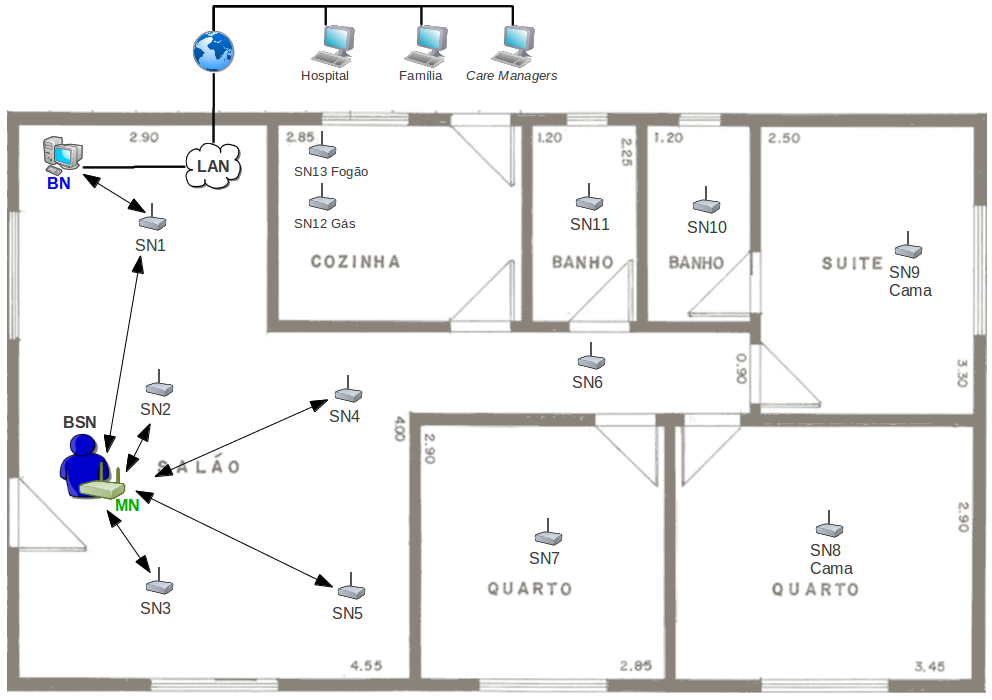
\includegraphics[width=1\textwidth]{img/05_emos_overview.png}
  \caption{Esquema modular do \textit{Elder Monitorization System} (EMoS).}
  \label{fig:1:emosOverview}
\end{figure}

O sistema \acs{EMoS} (Figura \ref{fig:1:emosOverview}) � caracterizado pelos seguintes tipos de dispositivos:

\begin{itemize}
\item N� M�vel (\acf{MN}): Monitoriza��o de pessoas e calibra��o do sistema;
\item N� Fixo (\acf{SN}): Envio de \textit{beacons} para localiza��o, comunica��o e monitoriza��o dom�stica;
\item N� Base (\acf{BN}): Gest�o central do sistema recebendo os dados de monitoriza��o ou pedidos do utilizador e enviando mensagens para a rede \acs{WSN} ou para o exterior atrav�s de uma \acs{LAN}.
\end{itemize}

Os n�s fixos est�o ligados � rede el�ctrica e enviam periodicamente  mensagens de assinatura em modo \textit{broadcast}. No caso dos n�s \textit{SN8}, \textit{SN9}, \textit{SN12} e \textit{SN13}, pode existir tamb�m envio de mensagens para outros n�s fixos ou para o n� base. Isto pode acontecer quando por exemplo, � detectado g�s no caso do \textit{SN12}, quando � ligado/desligado o fog�o no caso do \textit{SN13} ou quando algu�m se deita/levanta numa das camas onde est�o os sensores \textit{SN8} e \textit{SN9}.

O n� base recebe informa��o dos n�s fixos ou do exterior atrav�s da \acs{LAN} e toma decis�es com base nessa informa��o. Pode, por exemplo, avisar num monitor que existe alguma anomalia na casa, enviar uma mensagem para o n� m�vel ou para um n� fixo, ou comunicar com o exterior caso seja necess�rio. 

O n� m�vel pode funcionar em dois modos: calibra��o e normal. No modo de calibra��o limita-se a receber assinaturas dos n�s fixos e a registar essa informa��o, gerando um ficheiro XML com o mapa r�dio do casa. No modo normal recebe de igual forma as assinaturas, mas periodicamente envia de volta para o n� fixo mais pr�ximo, um conjunto de m�dias das pot�ncias recebidas. O n� fixo por sua vez envia esta informa��o para o n� base que ir� calcular a localiza��o do n� m�vel.

Todos os n�s formam uma estrutura em \textit{flat-routing} usando o \acs{AODV} para comunicar e apresentam uma estrutura interna id�ntica (Figura \ref{fig:2:emonsNodeInternal}). O sistema � perfeitamente escal�vel, sendo poss�vel adicionar-se v�rios outros n�s m�veis. No caso de existir um n�mero muito elevado de n�s m�veis, � poss�vel criar novos n�s base associados a \textit{clusters} de n�s fixos, que comuniquem atrav�s da LAN para eliminar sobreposi��es.

\begin{figure}[!htb]
  \centering
  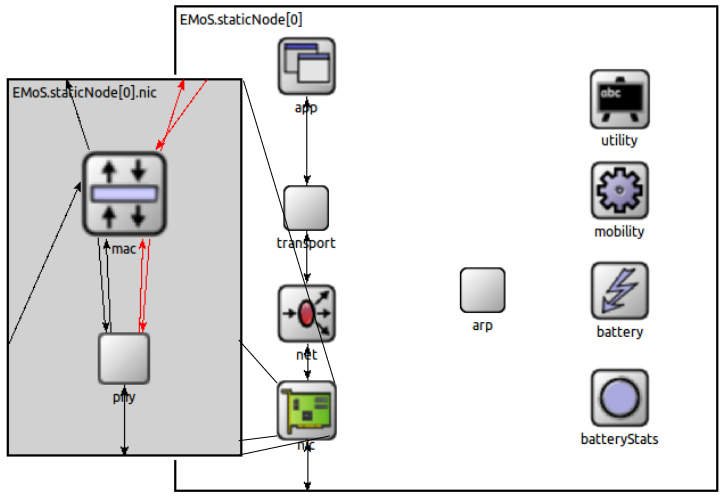
\includegraphics[width=0.78\textwidth]{img/05_emos_node_internal.png}
  \caption{Estrutura interna de um n� no sistema EMoS.}
  \label{fig:2:emonsNodeInternal}
\end{figure}

\clearpage

Neste trabalho foi criada uma camada \textit{Network} comum para todos os n�s e uma camada \textit{Application} por cada tipo de n� que implementa cada u dos tipos descritos. Nas pr�ximas sec��es � feita uma exposi��o detalhada de todo o sistema.

\subsection{N� M�vel (MN)}
\label{chap:5:sec:1.1}

O n� m�vel � um sensor equipado com r�dios \acs{IEEE} 802.15.4 e Bluetooth, um aceler�metro, um bot�o de p�nico e capacidade de armazenamento em cart�o \acs{SD}. O facto de ter dois tipos de r�dio permite-lhe comunicar com ambas as redes \acs{BSN} para monitoriza��o local biom�dica e \acs{WSN}. Est� instalado num objecto de uso di�rio, como uma bengala, um andarilho ou uma cadeira de rodas e possui baterias recarreg�veis. O carregamento � feito no s�tio habitual de apoio da bengala ou ent�o por liga��o com as baterias de uma cadeira de rodas el�ctrica.

A rede \acs{BSN} � composta por um electrocardi�grafo e um medidor de press�o arterial ambos equipados com Bluetooth, que efectuam monitoriza��o cont�nua. Quando detectam uma situa��o an�mala comunicam a mesma ao n� m�vel. Na simula��o este comportamento � recreado com um temporizador aleat�rio no n� m�vel que simula a comunica��o vinda da \acs{BSN} ao n�vel da aplica��o.

Como solu��o de hardware sugere-se a utiliza��o do m�dulo \textit{Waspmote} (Figura \ref{fig:3:waspMote}, com r�dio \textit{XBee-802.15.4} (Figura \ref{fig:4:waspXBee}), da \textit{Libelium}\footnote{http://www.libelium.com/products/waspmote} que permite a utiliza��o de dois tipos de r�dio, tem aceler�metro integrado, micro\acs{SD} e pins para obten��o do \acs{RSSI}. 

\begin{figure}[!htb]
  \centering
  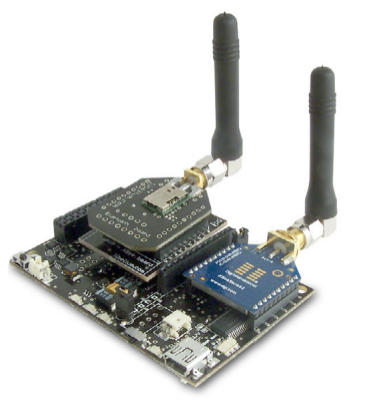
\includegraphics[width=0.57\textwidth]{img/05_wasp_mote.png}
  \caption{M�dulo \textit{Waspmote} da \textit{Libelium}.}
  \label{fig:3:waspMote}
\end{figure}

\begin{figure}[!htb]
  \centering
  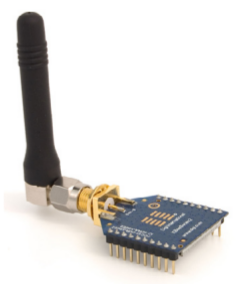
\includegraphics[width=0.40\textwidth]{img/05_wasp_xbee.png}
  \caption{R�dio \textit{XBee} IEEE 802.15.4 usado no m�dulo \textit{Waspmote}.}
  \label{fig:4:waspXBee}
\end{figure}

O r�dio \textit{XBee} simulado ter� os seguintes par�metros obtidos do  manual  \footnote{http://ftp1.digi.com/support/documentation/90000982\_H.pdf}): 

\begin{table}[!htb]
	\centering
\begin{tabular}{ |l|r|}
	\hline
  	Par�metro & Valor \\
  	\hline
  	Modulation & O-QPSK \\
  	Receiver Sensitivity & -92 dbM  \\
  	Transmit Power	& 1mW \\
  	Sleep Current & <10 uA \\
  	Current Consumption RX & 50 mA \\
  	Current Consumption TX (P=0dBm) & 45 mA \\
  	\hline
\end{tabular}
	\caption{Par�metros do r�dio \textit{XBee} da \textit{Digi}.}
	\label{tab:1:xbeeNICParameters}
\end{table}

\subsection{N� Fixo (SN)}
\label{chap:5:sec:1.2}

O n� fixo est� equipado com r�dio \acs{IEEE} 802.15.4. Ficar� ligado � rede el�ctrica dada a necessidade de estar periodicamente a enviar assinaturas em \textit{broadcast}. O hardware escolhido para a implementa��o deste n� ser� o \textit{MicaZ} com r�dio \textit{Texas Instruments CC2420} da \textit{Crossbow}\footnote{http://www.xbow.com/} (Figura \ref{fig:5:micaz}).

\begin{figure}[!htb]
  \centering
  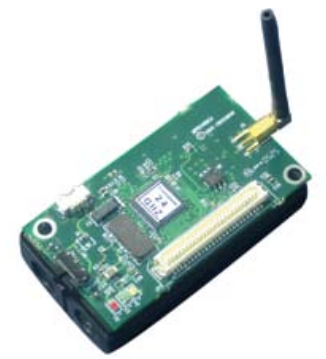
\includegraphics[width=0.35\textwidth]{img/05_micaz.png}
  \caption{M�dulo \textit{Micaz} da \textit{Crossbow}.}
  \label{fig:5:micaz}
\end{figure}

A escolha deste n� � motivada pelo baixo custo do mesmo e o facto de ser o n� que estar� presente em maior n�mero na rede.

O r�dio \textit{Texas Instruments CC2420} tem os seguintes par�metros obtidos do manual\footnote{http://www.ti.com/lit/gpn/cc2420};
\begin{table}[!htb]
	\centering
\begin{tabular}{ |l|r|}
	\hline
  	Par�metro & Valor \\
  	\hline
  	Modulation & O-QPSK \\
  	Receiver Sensitivity & -95 dBm  \\
  	Transmit Power & 1.1mW \\
  	Sleep Current & 0.02 uA \\
  	Current Consumption RX & 18.8 mA \\
  	Current Consumption TX (P=0dBm) & 17.4 mA \\
  	\hline
\end{tabular}
	\caption{Par�metros do r�dio \textit{Texas Instruments CC2420}.}
	\label{tab:2:CC2420NICParameters}
\end{table}

\subsection{N� Base (BN)}
\label{chap:5:sec:1.3}

O n� base tem como fun��o efectuar toda a gest�o centralizada da informa��o gerada por cada um dos sensores. Dada a grande necessidade de rapidez de processamento, espa�o de armazenamento e comunica��o com o exterior, optou-se por usar um \acs{PC} ligado a uma \acs{LAN} que est� por sua vez ligada � Internet. Assim o hardware para a implementa��o f�sica deste n� e que far� a ponte entre o \acs{PC} e a rede \acs{WSN}, ser� o \textit{Waspmote Gateway}, com r�dio \textit{XBee-802.15.4} (Figura \ref{fig:4:waspXBee}), da \textit{Libelium}. 

\begin{figure}[!htb]
  \centering
  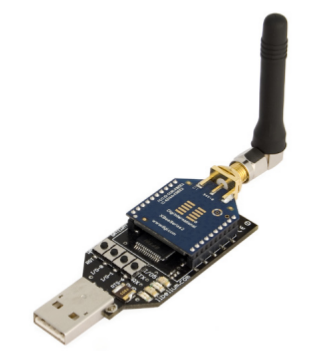
\includegraphics[width=0.40\textwidth]{img/05_waspmote_gateway.png}
  \caption{M�dulo \textit{Waspmote Gateway} da \textit{Libelium}.}
  \label{fig:6:waspmoteGateway}
\end{figure}

Este n� usa o mesmo r�dio que o \textit{Waspmote}, com par�metros para simula��o j� registados na Tabela \ref{tab:1:xbeeNICParameters}.

\clearpage

\section{Camada \textit{Network} : \textit{AODVRoute}}
\label{chap:5:sec:3}

A tecnologia ZigBee � hoje bastante usada nas redes \acs{WSN} com v�rios produtos para as mais diversas �reas. O ZigBee usa como primeiro protocolo na camada \textit{Network} o \acf{AODV} e seguidamente quando este falha um protocolo hier�rquico. Assim por forma a garantir uma compatibilidade do sistema desenvolvido com o ZigBee optou-se por implementar este protocolo no \acs{MiXiM}. 

O \acs{AODV} � um protocolo \textit{on-demand} que permite descobrir um caminho apenas quando este � necess�rio, recuperar caminhos perdidos e reutilizar caminhos j� encontrados. Achou-se por isso conveniente implement�-lo no \acs{MiXiM} para ser usado no \acs{EMoS}. Este usa caminhos bidireccionais, o que significa que quando � feita a descoberta de um novo caminho s�o sempre gerados dois, acelerando o processo de procura de novos caminhos. A utiliza��o de contadores sequenciais impede e forma��o de loops em todo o processo e � feita manuten��o sobre os caminhos para eliminar os que deixaram de ser usados durante um determinado espa�o de tempo.

Neste trabalho foi implementada uma vers�o do \acs{AODV} que apenas cont�m as funcionalidades necess�rias para descoberta de um novo caminho ou para a recupera��o de um caminho perdido. O \textit{multicast} bem como a repara��o local de caminhos perdidos (\textit{local-repair}\footnote{repara��o que ocorre localmente quando um n� interm�dio falha no encaminhamento da mensagem.}) n�o foram implementadas. Ao m�dulo implementado foi dado o nome de \textit{AODVRoute}.

\subsection{Tipos de Mensagens}
\label{chap:5:sec:3.1}
O \acs{AODV} funciona utilizando pelo menos tr�s tipos de mensagens para descobrir o caminho de um n� A para um n� B.

\begin{itemize}
\item \acf{RREQ};
\item \acf{RREP};
\item \acf{RERR}.
\end{itemize}

Pode ainda existir um quarto tipo de mensagem, opcional, o \acf{RREP-ACK}, utilizado quando existe o perigo de existirem liga��es unidireccionais que impe�am a chegada de um \acs{RREP}, mas que n�o ser� referido neste trabalho.

\begin{figure}[!htb]
  \centering
  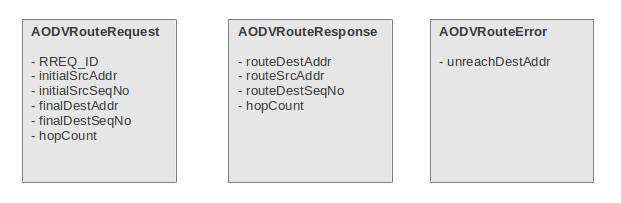
\includegraphics[width=1\textwidth]{img/05_aodv_msg_types.png}
  \caption{Tipos de mensagens do AODVRoute.}
  \label{fig:11:aodvMsgTypes}
\end{figure}

Na Figura \ref{fig:11:aodvMsgTypes} est�o as mensagens criadas no \acs{MiXiM}. A cria��o de mensagens no \acs{OMNeT++} � relativamente simples uma vez que todo o \textit{boilerplate code} � gerado automaticamente. Assim � necess�rio apenas definir ficheiros do tipo \textit{msg} com os par�metros necess�rios. Cada uma das mensagens definidas para este m�dulo estende a mensagem \textit{NetwPkt}, uma mensagem gen�rica para a camada \textit{Netw} com endere�os de emissor e receptor e \acf{TTL}. Para al�m dos campos herdados existem tamb�m os seguintes campos para cada tipo de mensagem:

\begin{itemize}
\item \textit{AODVRouteRequest} : endere�os e n�meros de sequ�ncia para o n�s emissor e receptor, o \textit{RREQ\_ID} que � obtido de um contador existente para o efeito no n� emissor e o contador de saltos que permite perceber em que ponto do caminho est� o \acs{RREQ};
\item \textit{AODVRouteResponse} : endere�os de emissor e receptor, n�mero de sequ�ncia do n� de receptor e n�mero de saltos at� ao receptor;
\item \textit{AODVRouteError} : endere�o do n� de destino que n�o foi encontrado. 
\end{itemize}

\subsection{Estruturas de Dados}
\label{chap:5:sec:3.2}

Foram criadas tr�s estruturas de dados neste novo m�dulo:

\begin{itemize}
\item \textit{pktMap} : utilizada para guardar os pacotes que vieram da camada \acs{APP} por n� de destino, num \acs{FIFO} quando para estes ainda n�o existe um caminho encontrado;
\item \textit{RREQVector} : utilizada para guardar os pacotes \acs{RREQ} recebidos;
\item \textit{routeMap} :utilizada para guardar as rotas em cada n� e a lista de precursores\footnote{Precursor de um caminho, � um n� que antecede o n� actual no caminho e s� existe depois de ter enviado pelo menos uma mensagem pelo n� actual.} dessa rota.
\end{itemize}

\begin{figure}[!htb]
  \centering
  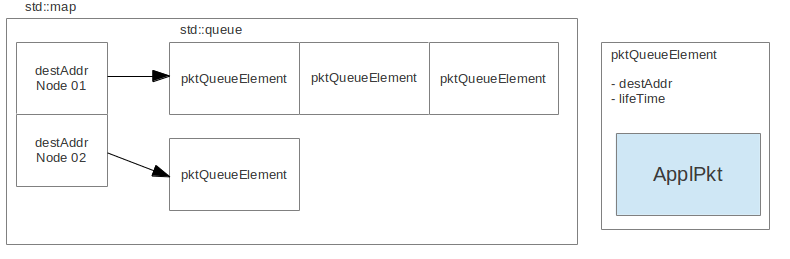
\includegraphics[width=1\textwidth]{img/05_aodv_pkt_map.png}
  \caption{PktMap - estrutura para a gest�o dos pacotes de aplica��o em espera.}
  \label{fig:8:aodvPktMap}
\end{figure}

Na Figura \ref{fig:8:aodvPktMap} observamos a estrutura PktMap. Este mapa de pares do tipo de endere�os e filas de pacotes, guarda para cada n� de destino os pacotes em espera de um caminho para o seu destino final. Cada elemento da fila tem como par�metros o endere�o do n� de destino, o tempo de vida do elemento (\begin{math}t_0+t\end{math}) e o pacote que foi enviado da camada \acs{APP}. Esta estrutura � sujeita a uma manuten��o peri�dica que elimina os todos os elementos para os quais \begin{math}t_{sim}>lifetime\end{math}. O tempo de vida � suficientemente curto para que n�o exista uma disparidade grande entre o momento que foi encontrado um caminho e a nova posi��o do n� m�vel.

\begin{figure}[!htb]
  \centering
  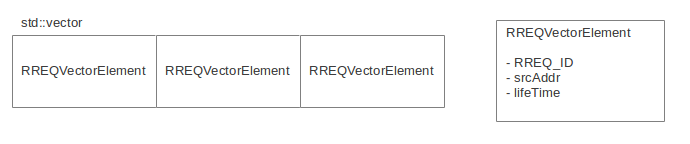
\includegraphics[width=1\textwidth]{img/05_aodv_rreq_vector.png}
  \caption{RREQVector - estrutura que guarda os RREQs recebidos num n�.}
  \label{fig:9:aodvRREQVec}
\end{figure}

Na Figura \ref{fig:9:aodvRREQVec} observamos a \textit{RREQVec}, estrutura que guarda a chave pares \textit{RREQ\_ID} e \textit{srcAddr}, por forma a distinguir univocamente todos os \acp{RREQ} recebidos de um determinado n� evitando assim o envio de um \acs{RREQ} que j� foi anteriormente enviado.

\begin{figure}[!htb]
  \centering
  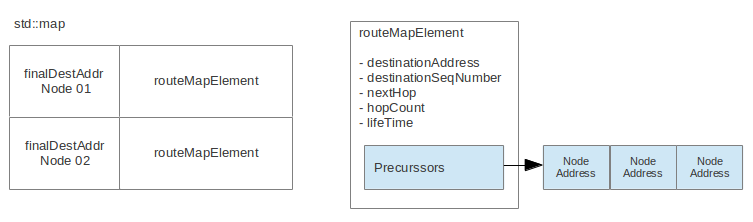
\includegraphics[width=1\textwidth]{img/05_aodv_route_map.png}
  \caption{RouteMap - estrutura que guarda os caminhos encontrados para n�s destino.}
  \label{fig:10:aodvPktMap}
\end{figure}

Finalmente na Figura \ref{fig:10:aodvPktMap} temos a estrutura \textit{RouteMap} que guarda a informa��o dos caminhos encontrados em cada n�. Est�o presentes em cada \textit{routeMapElement}, o n� final de destino do caminho, o n�mero de sequ�ncia conhecido do destino, o pr�ximo n� do caminho, o n�mero de n�s entre o n� actual e o n� de destino, o tempo de vida do caminho usado para garantir que os caminhos que deixaram de ser usados n�o ficam a ocupar espa�o no limitado armazenamento dispon�vel e uma lista de n�s precursores que servir� para para enviar um \acs{RERR} de volta para todos os n�s que anteriormente usaram o caminho que deixou de existir.

\subsection{Modo de Funcionamento}
\label{chap:5:sec:3.3}

Neste trabalho a camada de aplica��o poder� gerar v�rios tipos de mensagens. Essas mensagens poder�o ser em \textit{broadcast} no caso das mensagens de assinatura enviadas pelos n�s fixos ou \textit{unicast} quando existe um n� que pretende comunicar com outro. Todos os n�s do sistema \acs{EMoS} podem comunicar uns com os outros, no entanto, nem sempre de forma directa. Sendo a camada \textit{Network} comum a todos os n�s o comportamento � id�ntico para todos. 

Suponhamos que a camada de aplica��o de um n� fixo pretende enviar uma mensagem para o n� base, informando que o existe uma fuga de g�s. A partir desse momento � mensagem de aplica��o � anexada informa��o de controlo (\textit{NetwControlInfo}), contendo o endere�o \textit{Network} do n� de destino, sendo enviada para a camada abaixo. A mensagem segue ent�o o fluxograma da Figura \ref{fig:12:aodvFlux1}. De notar que o caso em que o endere�o de destino � igual ao do pr�prio n�, decorre de um erro de atribui��o do endere�o final na camada de aplica��o. A incrementa��o da sequ�ncia do n� � feita para o caso de ainda existir \acp{RREQ} perdidos no ambiente.

\begin{figure}[!htb]
  \centering
  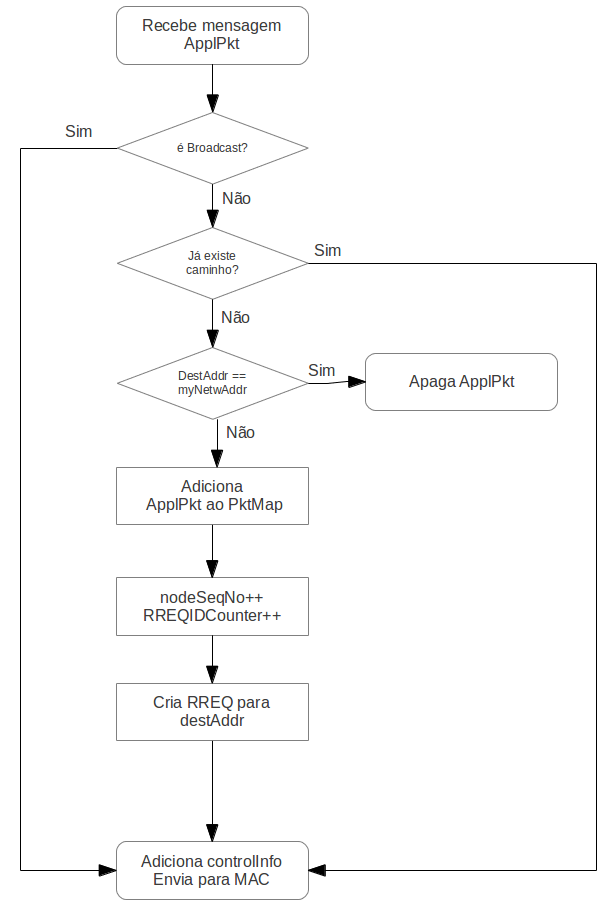
\includegraphics[width=0.9\textwidth]{img/05_aodv_flow_01.png}
  \caption{Fluxograma de chegada da mensagem de aplica��o � camada \textit{Network}.}
  \label{fig:12:aodvFlux1}
\end{figure}

Cada n� guarda tamb�m um registo, para cada n� com o qual j� tenha comunicado um registo do n�mero de sequ�ncia desse n�. Este valor � colocado no \acs{RREQ} para que, caso seja encontrado um caminho mais recente, este pedido seja ignorado.

Portanto quando n�o existe caminho para o n� pretendido de destino, o n� de origem gera o \acs{RREQ} que � enviado em modo \textit{broadcast} para o resto da rede. Na Figura \ref{fig:13:aodvFlux2} est� a recep��o de outro n� do pacote enviado pelo n� de origem. 

\begin{figure}[!htb]
  \centering
  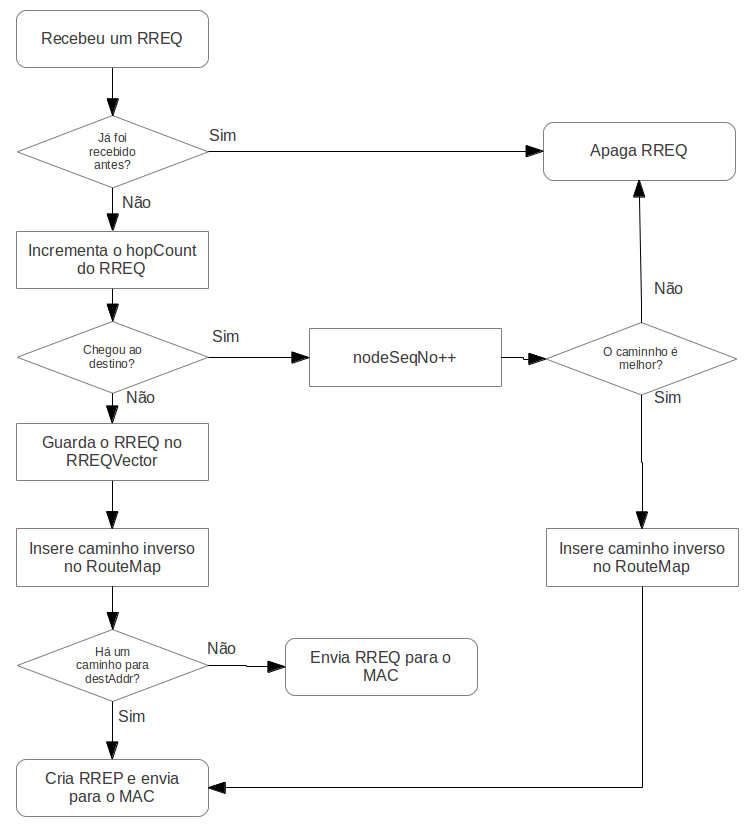
\includegraphics[width=1\textwidth]{img/05_aodv_flow_02.png}
  \caption{Fluxograma de chegada de um \textit{RREQ} vindo da camada \textit{MAC}.}
  \label{fig:13:aodvFlux2}
\end{figure}


Dado que o n� guarda todos os \acs{RREQ} que recebe no \textit{RouteVector}, este consegue verificar se j� recebeu aquele mesmo pacote ou n�o. No caso de n�o ter recebido � incrementado o contador de saltos para que a dist�ncia at� � origem seja actualizada. A informa��o do n� de origem, o n�mero de saltos at� ao mesmo s�o usados para criar um caminho inverso para o n� de origem. Enquanto este n�o for o n� de origem a mensagem vai sendo enviada de n� para n� at� chegar ao destino. Pode ainda se dar o caso do n� n�o ser o n� de destino mas j� existir um caminho no \textit{RouteMap}, o que permite ao n� interm�dio devolver logo um \acs{RREP}. Quando se trata do n� de destino, � incrementado o contador do n� para garantir que n�o haver� mais nenhum caminho que se sobreponha.  

Ent�o, assim que o caminho � encontrado, existe um \acs{RREP} que volta pelo caminho inverso em \textit{unicast} construindo o caminho do n� de origem para o n� de destino iniciais. 

\clearpage

Na Figura \ref{fig:14:aodvFlux3} podemos observar o que acontece a essa mensagem � medida que vai passando pelos n�s interm�dios at� chegar ao n� de origem original. Quando � alcan�ada a origem, o n� pode ent�o ir buscar ao pktMap, a pr�xima mensagem e envi�-la para aquele endere�o de destino.

\begin{figure}[!htb]
  \centering
  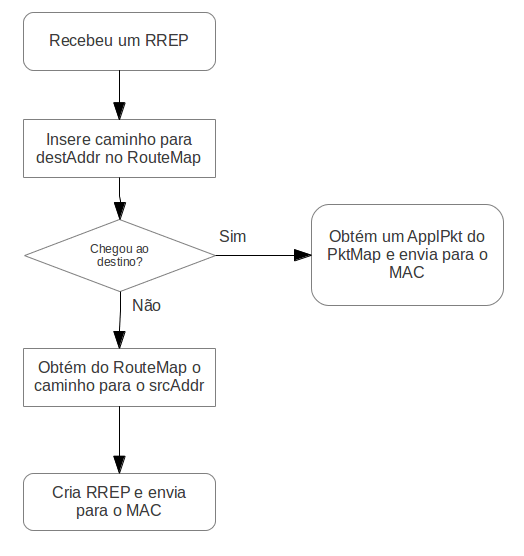
\includegraphics[width=0.7\textwidth]{img/05_aodv_flow_03.png}
  \caption{Fluxograma de chegada de um \textit{RREP} vindo da camada \textit{MAC}.}
  \label{fig:14:aodvFlux3}
\end{figure}

Quando ocorre um erro, ou seja, existe uma mensagem que � entregue mas o \acs{MAC} n�o recebe uma resposta de confirma��o \acs{ACK}, � necess�rio tomar medidas para que a origem seja informada que aquele caminho j� n�o � v�lido. Assim s�o criados \acs{RERR} que viajam pelos precursores at� atingir n� de origem. Na Figura \ref{fig:15:aodvFlux4} podemos ver a primeira fase quando a falha na entrega da mensagem ocorre. Nesse momento o n� procura todos os caminhos que estejam no \textit{RouteMap} e elimina-os, enviando depois um \acs{RERR} para cada um dos precursores.

\begin{figure}[!htb]
  \centering
  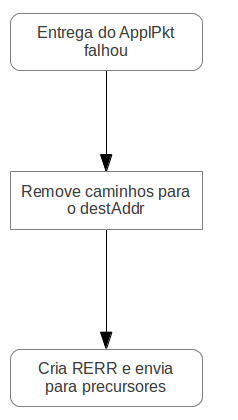
\includegraphics[width=0.33\textwidth]{img/05_aodv_flow_04.png}
  \caption{Fluxograma de chegada de uma mensagem de controlo com o pacote cuja entrega falhou no \textit�{MAC}.}
  \label{fig:15:aodvFlux4}
\end{figure}

Na Figura \ref{fig:16:aodvFlux5}  temos o comportamento dos n�s interm�dios e destino (origem do caminho eliminado). De notar que a mensagem vai sendo apagada, n� a n�, quando para cada percurso na �rvore j� n�o existem mais percursores.

\begin{figure}[!htb]
  \centering
  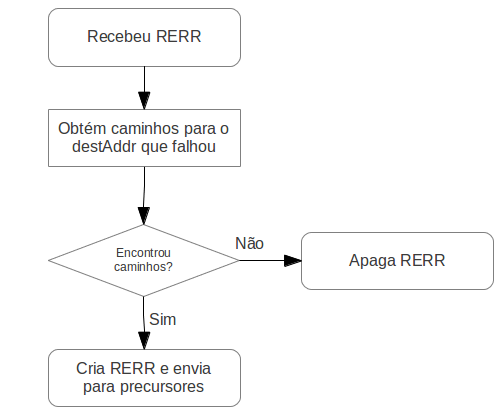
\includegraphics[width=0.70\textwidth]{img/05_aodv_flow_05.png}
  \caption{Fluxograma da chegada de um \textit{RERR} vindo da camada \textit{MAC}.}
  \label{fig:16:aodvFlux5}
\end{figure}

\clearpage

\section{Camada \textit{Application} : Localiza��o}
\label{chap:5:sec:4}

O sistema \acs{EMoS} usa para a localiza��o o m�todo \textit{HORUS} \cite{31} com algumas modifica��es que ser�o descritas na Sec��o \ref{chap:5:sec:4.1}. � um processo probabil�stico com precis�o elevada, raz�o pela qual foi escolhido para este trabalho. O processo  foi implementando completamente ao n�vel da camada de aplica��o e � constitu�do por duas fases distintas:

\begin{itemize}
\item Fase \textit{Offline} : fase onde � obtido o mapa r�dio e criados os \textit{clusters}. O n� m�vel (\acs{MN}) � configurado em modo de calibra��o e guarda numa estrutura de dados, as assinaturas recebidas vindas dos diversos n�s fixos que est�o � dist�ncia de recep��o. No fim da simula��o s�o criados dois ficheiros \textit{XML} que guardam posi��es ou \textit{clusters}. Esses ficheiros ser�o posteriormente interpretados pelo n� base.
\item Fase \textit{Online} : fase em que os n� m�veis enviam periodicamente mensagens com um conjunto de m�dias das pot�ncias recebidas dos v�rios n�s fixos para o n� base. Utilizando o mapa r�dio entretanto criado o n� base efectua o c�lculo da posi��o seleccionando primeiramente um \textit{cluster} de posi��es e depois calculando a probabilidade de cada posi��o.
\end{itemize}

\subsection{HORUS Modificado}
\label{chap:5:sec:4.1}

O sistema \textit{HORUS} usado no \acs{EMoS} difere do apresentado pelo seu autor em \cite{31}, na medida em que o c�lculo da posi��o n�o � feito no n� m�vel mas sim no n� base, sendo a correla��o entre amostras a �nica opera��o que permanece no dispositivo m�vel. Esta op��o de arquitectura deveu-se �s seguintes raz�es:

\begin{itemize}
\item Poupan�a de bateria no n� m�vel;
\item Fraca capacidade de processamento do n� m�vel;
\item Necessidade de centraliza��o das posi��es de v�rios n�s m�veis num �nico s�tio podendo assim ser feita a correla��o de resultados vindos de todos os n�s;
\item Complexidade do sistema de localiza��o.
\end{itemize}

\begin{figure}[!htb]
  \centering
  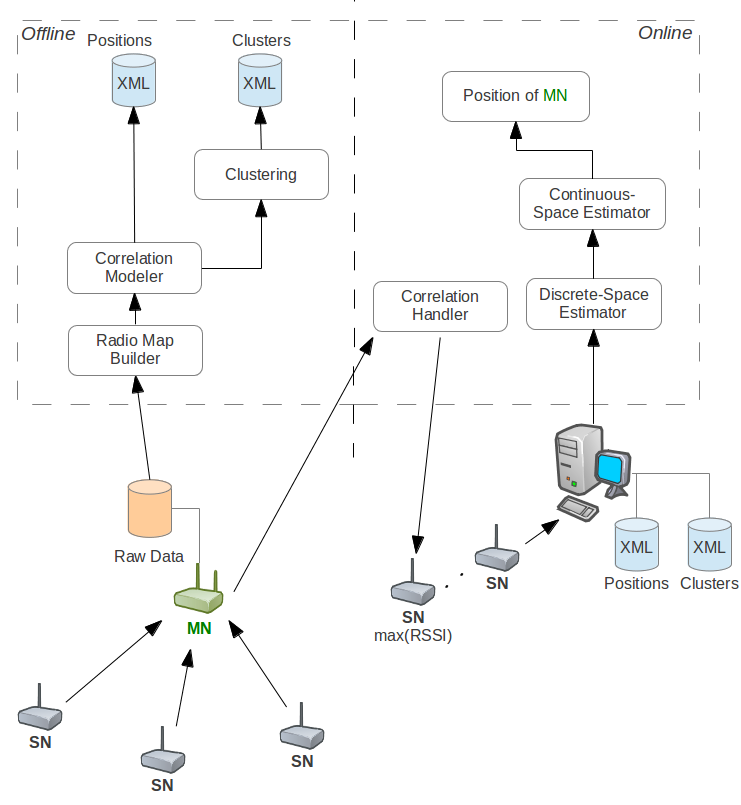
\includegraphics[width=0.85\textwidth]{img/05_horus_mod.png}
  \caption{Componentes do sistema HORUS modificado e fluxo de informa��o.}
  \label{fig:17:horusMod}
\end{figure}

\title{\textbf{\textit{Fase Offline}}}

Na Figura \ref{fig:17:horusMod} � descrito de forma global e modular todo o sistema de localiza��o implementado. Na fase \textit{offline} o n� m�vel recolhe para cada posi��o da casa uma s�ries de amostras (\textit{Raw Data}),pares (nodeAddress,RSSI) obtidos a partir da informa��o de controlo enviada pela camada \textit{Network}. Esta informa��o vai sendo guardada, sem qualquer tratamento, para todas as posi��es registadas. 

Depois de conclu�da a amostragem de todo o espa�o a informa��o � agrupada por posi��o no \textit{Radio Map Builder} e correlacionada efectuando para cada posi��o e para cada n�, o c�lculo da m�dia e do desvio padr�o, das pot�ncias recebidas no \textit{Correlation Modeler}. Em cada posi��o � mantido um n�mero m�ximo configur�vel de n�s registados, sendo todos os outros removidos, pretendendo-se com isto garantir que na fase \textit{Online} as amostras recebidas s�o cruzadas com amostras do mesmo tamanho para cada posi��o.

Por fim � feita a cria��o de \textit{clusters} no m�dulo \textit{Clustering}. O processo decorre ordenando por pot�ncia recebida as amostras para cada posi��o e depois escolhendo as \begin{math}n\end{math} primeiras como chave da posi��o. Para cada chave diferente � criado um novo \textit{cluster}. De notar que a chave (1000,1001) � igual � chave (1001,1000) n�o havendo o conceito de ordena��o na chave. Neste trabalho considerou-se \begin{math}n=2\end{math} por ser um valor apontado no trabalho \cite{31} como tendo bons resultados num sistema real.

Para efeitos de simula��o este comportamento foi emulado usando o m�dulo de mobilidade \textit{TractorMobility} disponibilizado pelo \acs{MiXiM} e descrito na Sec��o \ref{chap:5:sec:5}.Foram registadas posi��es separadas na horizontal por 1 metro e na vertical por 2 metros para toda a �rea de trabalho, em per�odos de 40 segundos. Ap�s cada mudan�a de posi��o, o n� m�vel simulado calcula a m�dia e o desvio padr�o dos valores de \acs{RSSI} recebidos e guarda numa estrutura de dados de posi��es  \textit{radioMap} (ver Sec��o \ref{chap:5:sec:4.2}). Quando a simula��o termina o \textit{radioMap} � transformado num ficheiro XML e s�o criados os \textit{clusters} da forma descrita no par�grafo anterior, que tamb�m s�o transformados num ficheiro XML.

\title{\textbf{\textit{Fase Online}}}

Nesta fase o n� m�vel recolhe e guarda assinaturas dos n�s fixos durante um determinado tempo. Ap�s esse momento usa o \textit{Correlation Handler} para efectuar uma m�dia por n� fixo, das diversas pot�ncias recebidas. Esse resultado � enviado para o n� com o o maior valor de \acs{RSSI} detectado at� esse momento. O n� fixo reconhece o tipo de mensagem e envia directamente ou atrav�s de outros n�s fixos, a mensagem para o n� base.  

O n� base cont�m os ficheiros XML gerados na fase \textit{offline} e como tal possui toda a informa��o necess�ria para determinar a probabilidade do n� estar numa determinada posi��o. Inicialmente a estimativa � discreta (\textit{Discrete-Space Estimator}) e apenas s�o determinadas posi��es para o n� m�vel que constam no mapa r�dio. 

Nesse momento o n� fixo analisa o sinal recebido, verifica se est�o presentes um n�mero m�nimo de n�s fixos e determina a chave da amostra (neste caso os dois n�s com maior \acs{RSSI}). Com essa chave obt�m o \textit{cluster} correspondente e as posi��es associadas. Para cada posi��o � calculada a densidade de probabilidade da distribui��o normal (Ver Sec��o \ref{chap:5:sec:4.2}). A posi��o com maior valor � a posi��o obtida � sa�da do \textit{Discrete-Space Estimator}.

Uma vez que existem diversas posi��es onde o n� m�vel poder� estar, que n�o est�o registadas no mapa r�dio � necess�ria uma estima��o no espa�o cont�nua. � essa precisamente a fun��o do \textit{Continuous-Space Estimator} que ir� atrav�s de duas t�cnicas: centro de massa das posi��es e m�dia temporal do espa�o f�sico, determinar uma posi��o estimada da posi��o real do n�.

\subsection{Modelo Matem�tico}
\label{chap:5:sec:4.2}

O sistema \textit{HORUS} � um m�todo probabil�stico.Neste trabalho optou-se pela parametriza��o do sinal recebido, que permite obter uma distribui��o normal que se ajusta ao histograma das pot�ncias recebidas tal como podemos ver na Figura \ref{fig:23:horusNormal}.

\begin{figure}[!htb]
  \centering
  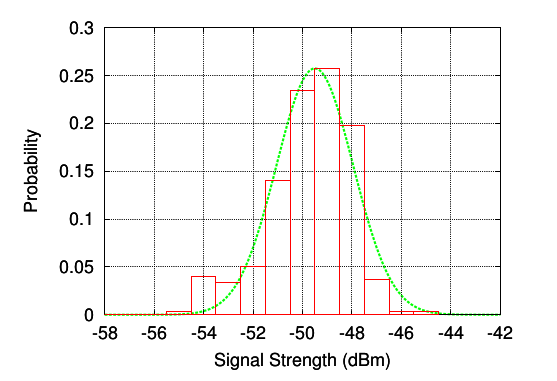
\includegraphics[width=0.8\textwidth]{img/05_horus_normal.png}
  \caption{Exemplo de parametriza��o da distribui��o de pot�ncia do sinal recebido \cite{31}.}
  \label{fig:23:horusNormal}
\end{figure}

A fun��o densidade de probabilidade da distribui��o normal � dada por:

\begin{equation}
fdp(q) = \frac{1}{\sigma{}\sqrt{2\pi{}}}e^\frac{-(q-\mu)^2}{2\sigma{}^2}
\label{eq1}
\end{equation}

Para \begin{math}n\end{math} amostras recebidas por um n� fixo \begin{math}i\end{math} os par�metros de  \eqref{eq1} s�o obtidos, calculando a m�dia e o desvio padr�o das amostras obtidas, usando as equa��es \ref{eq2} e \ref{eq3}.

\begin{equation}
\mu{} = \frac{1}{n}\sum_{j=1}^{n} s_i(j)\
\label{eq2}\
\end{equation}

\begin{equation}
\sigma{} = \sqrt{\frac{1}{n}\sum_{j=1}^{n}(s_i(j)-\mu{})^2}
\label{eq3}
\end{equation}

onde \begin{math}s_i(j)\end{math} � a amostra \begin{math}j\end{math} proveniente do n� fixo \begin{math}i\end{math}.

O facto de se aproximar as amostras a uma fun��o densidade de probabilidade permite uma poupan�a significativa de espa�o de armazenamento, uma vez que deixa de ser necess�rio guardar os valores das pot�ncias recebidas. Para cada par (n�,posi��o) passa por isso a ser necess�rio guardar apenas a m�dia e desvio padr�o da fun��o. Esta abordagem permite tamb�m obter valores de probabilidade para pot�ncias de sinal que n�o tenham sido medidas e filtrar poss�veis anomalias registadas durante a fase \textit{offline}. 

Na fase \textit{online} � necess�rio calcular a probabilidade de um n� estar numa determinada posi��o. Assim � necess�rio para um vector \begin{math}s=(s_1,...,s_k)\end{math} encontrar a posi��o \begin{math}x\end{math} que maximiza a probabilidade \begin{math}P(x/s)\end{math}. Para obter esta probabilidade usando a fun��o densidade de probabilidade entretanto guardada recorremos � equa��o:

\begin{equation}
P(s_i/x) =  P(s_i<=0.5) = \int_{s_i-0.5}^{s_i+0.5} fdp(q) dq
\label{eq4}
\end{equation}

Dado que queremos evitar a utiliza��o de algoritmos num�ricos, computacionalmente pesados, para a resolu��o do integral, transformou-se a fun��o densidade de probabilidade encontrada para cada n� est�tico, numa fun��o de distribui��o normal standard, cujos valores podem ser tabelados. Para efeitos de simula��o criou-se por isso, um ficheiro XML que cont�m os valores necess�rios.

Assim sabendo que:

\begin{equation}
P(X<=x) = P(\frac{X-\mu{}}{\sigma{}} <= \frac{x-\mu{}}{\sigma{}}) = P(Z<=z)
\end{equation}

onde \begin{math}Z\end{math} � uma vari�vel normal aleat�ria standard, podemos calcular a probabilidade da \eqref{eq4} como:

\begin{equation}
P(s_i<=0.5) = P(Z<=\frac{s_i+0.5-\mu{}_i}{\sigma{}_i})
\end{equation}

onde com os valores tabelados rapidamente chegamos a um resultado.

Para um amostra que contenha v�rios n�s est�ticos, a probabilidade conjunta � dada pela multiplica��o das probabilidades individuais calculadas para cada n�:

\begin{equation}
P = \prod_{j=1}^{n} P_i
\end{equation}

Obtida uma posi��o usando o \textit{Discrete-Space Estimator} torna-se necess�rio ainda usar o \textit{Continous-Space Estimator} para chegar a um valor mais pr�ximo da localiza��o real.

A primeira t�cnica � o centro de massa de \begin{math}N\end{math} posi��es obtidas. A posi��o estimada no espa�o cont�nuo \begin{math}(x,y)\end{math} � obtida a partir das seguintes equa��es, considerando o espa�o bi-dimensional utilizado neste trabalho:

\begin{equation}
x = \frac{\sum_{j=1}^{min(N,P)} x_iP_i}{\sum{}P_i}
\end{equation}
\begin{equation}
y = \frac{\sum_{j=1}^{min(N,P)} y_iP_i}{\sum{}P_i}
\end{equation}

Onde \begin{math}P\end{math} � o n�mero de posi��es encontradas para um determinado n� m�vel.

A segunda t�cnica consiste em fazer uma m�dia temporal das \begin{math}K\end{math} posi��es encontradas numa localiza��o anterior para o mesmo n�, dada pelas equa��es:

\begin{equation}
x = \frac{\sum_{j=1}^{K} x_i}{K}
\end{equation}
\begin{equation}
y = \frac{\sum_{j=1}^{K} y_i}{K}
\end{equation}

Neste trabalho ser�o usados os valores de base \begin{math}N=6\end{math} e \begin{math}K=10\end{math} referenciados em \cite{31} como valores com bons resultados numa situa��o real. Ser�o no entanto, obtidos resultados na simula��o, de modo a aferir quais os valores que d�o origem aos melhores resultados.

\subsection{Estruturas de Dados e Ficheiros XML}
\label{chap:5:sec:4.3}
S�o definidas duas estruturas de dados no \textit{HORUS} modificado.

Na Figura \ref{fig:18:horusModRadioMap} temos a estrutura de dados escolhida para guardar as posi��es obtidas � sa�da do \textit{Correlation Modeler}. O resultado � um conjunto de posi��es, onde para cada posi��o, existem v�rias fun��es de densidade de probabilidade para cada n�, \acfp{PDF} caracterizadas pelos seus valores de m�dia e desvio padr�o.

Na Figura \ref{fig:19:horusModRadioMapClusters} est� representada a estrutura de dados utilizada para guardar os \textit{clusters}. 

Estas estruturas est�o presentes no n� m�vel e no n� fixo e servem para guardar em mem�ria o conte�do que ser� escrito ou lido nos ficheiros XML.Nesta simula��o s�o, por isso, usados dois tipos de ficheiro XML para guardar o mapa r�dio de posi��es e os \textit{clusters}. Estes ficheiros s�o gerados quando termina a simula��o do modo \textit{offline} e carregados pelo n� base quando come�a a simula��o do modo \textit{online}. No Anexo \ref{list:a1:xmlRadioMap} est� um exemplo de um ficheiro XML de posi��es r�dio e no Anexo \ref{list:a1:xmlRadioMapCluster} pode ser consultado um exemplo de um ficheiro XML de clusters.

\begin{figure}[!htb]
  \centering
  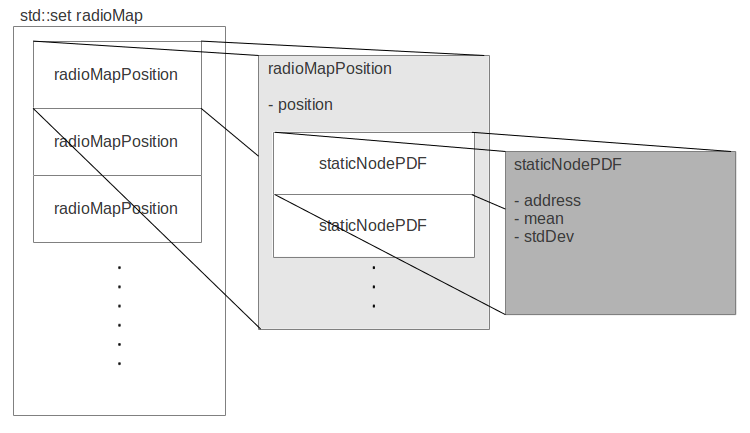
\includegraphics[width=1\textwidth]{img/05_horus_mod_radio_map.png}
  \caption{Estrutura de dados para armazenamento das posi��es do mapa r�dio obtidas na fase \textit{offline}.}
  \label{fig:18:horusModRadioMap}
\end{figure}

\begin{figure}[!htb]
  \centering
  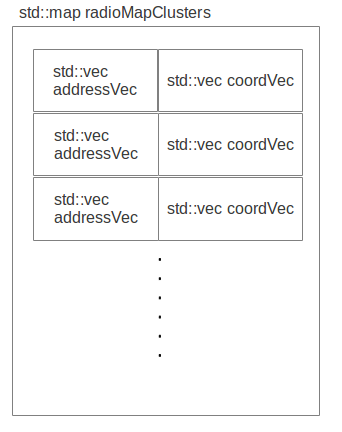
\includegraphics[width=0.4\textwidth]{img/05_horus_mod_radio_map_clusters.png}
  \caption{Estrutura de dados para armazenamento dos \textit{clusters} obtidos na fase \textit{offline}.}
  \label{fig:19:horusModRadioMapClusters}
\end{figure}

\subsection{Modo de Funcionamento}
\label{chap:5:sec:4.4}
Na camada de aplica��o dos n�s pertencentes ao \acs{EMoS} � definido o papel do n� da rede. Cada n� tem a sua camada pr�pria, o que em termos reais corresponderia a um programa em \textit{nesC} a ser executado sobre o \textit{TinyOS}. 

O n� m�vel e o n� base, t�m ambos um papel fulcral na localiza��o. Apresentam-se por isso nas Figuras \ref{fig:20:horusFlow01} e \ref{fig:21:horusFlow02} os fluxogramas correspondentes ao funcionamento da camada de aplica��o desses n�s no contexto da localiza��o.

\begin{figure}[!htb]
  \centering
  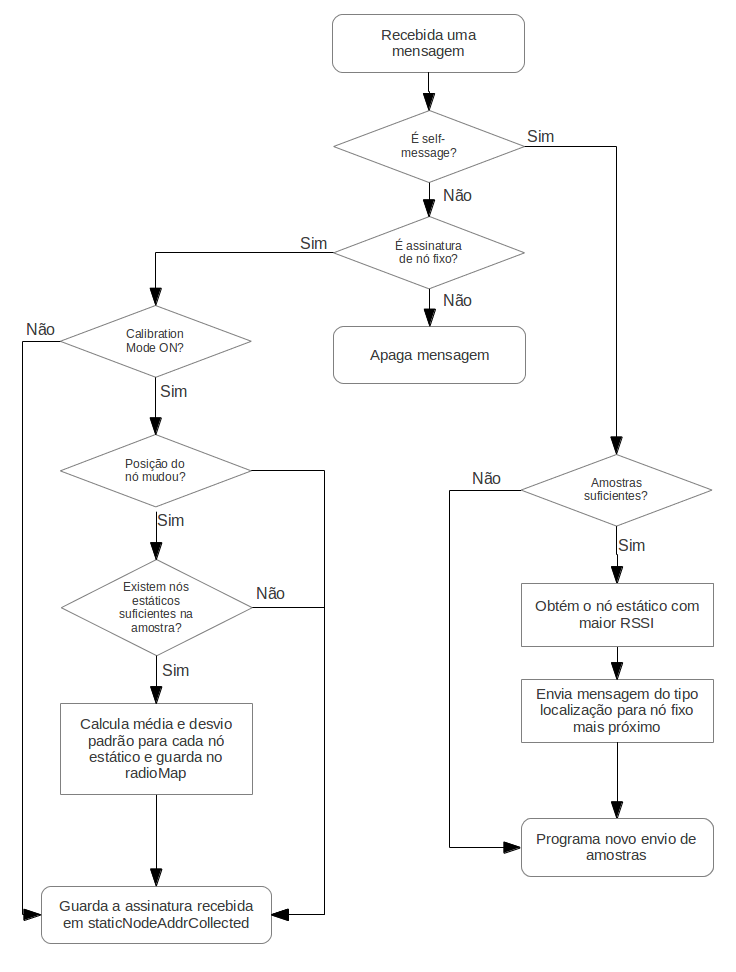
\includegraphics[width=1\textwidth]{img/05_horus_flow_01.png}
  \caption{Fluxograma do modo de funcionamento do n� m�vel na localiza��o.}
  \label{fig:20:horusFlow01}
\end{figure}

No fluxograma da Figura \ref{fig:20:horusFlow01} observamos o comportamento do n� m�vel. Este n� est� permanentemente a receber e guardar mensagens de assinatura vindas dos n�s fixos espalhados pela casa. 

No ramo esquerdo do fluxograma podemos observar o que acontece quando uma assinatura de um n� fixo � recebida. Se o n� m�vel estiver em modo de calibra��o, utilizado durante a fase \textit{offline}, o n� verifica se houve mudan�a de posi��o e se existem n�s est�ticos suficientes para considerar a posi��o v�lida. Caso tal aconte�a s�o calculados os par�metros da fun��o densidade de probabilidade normal correspondente �s pot�ncias amostradas (calculando-se a m�dia e o desvio padr�o) sendo o resultado guardado no mapa r�dio. Pelo contr�rio se estivermos na fase \textit{online} s�o apenas registados os valores do endere�o e pot�ncia de sinal recebidos.

Quando n�o est� no modo de calibra��o, o n� m�vel usa um conceito de agendamento do \acs{OMNeT++} que permite agendar eventos, atrav�s de mensagens que s�o enviadas, num determinado tempo da simula��o, para o pr�prio n�. Assim este conceito � usado para enviar periodicamente mensagens para o n� base para que este possa calcular a posi��o do n� m�vel. Este comportamento est� exemplificado na ramo direito do fluxograma.

\clearpage

Por sua vez na Figura \ref{fig:21:horusFlow02} temos um fluxograma do modo de funcionamento do n� base. Este n� recebe de um n� m�vel, por interm�dio de um ou mais n�s fixos, uma mensagem que cont�m as m�dias das pot�ncias de n�s fixos, recebidas pelo n� m�vel durante um determinado espa�o de tempo. Assim quando o n� base recebe esta mensagem, ordena por pot�ncia de forma descendente e selecciona apenas os N primeiros, em que N representa o n�mero de n�s est�ticos presentes em cada posi��o do mapa r�dio. 

S�o ent�o seleccionados os endere�os dos dois primeiros n�s est�ticos da amostra que constituem a chave da amostra. Com a chave s�o obtidas as posi��es do \textit{cluster} cuja chave � igual � chave da amostra. Percorrendo ent�o todas as posi��es obtidas � calculada para cada uma, a probabilidade do n� m�vel estar nessa posi��o.

Se a probabilidade for maior que zero ent�o � guardada numa lista. Uma vez percorridos todas as posi��es se ainda n�o houver na lista pelo menos uma posi��o, decrementa-se o valor de N e torna-se a obter as posi��es do \textit{cluster} para novo c�lculo. Se N chegar a zero ent�o o processo acaba sem conseguir determinar uma posi��o para o n� m�vel. Se houver uma posi��o ent�o � efectuada a estima��o de espa�o cont�nuo atrav�s do centro de massa das posi��es e � calculada a m�dia temporal de espa�o cont�nuo com as �ltimas posi��es calculadas em amostras anteriores.

\begin{figure}[!htb]
  \centering
  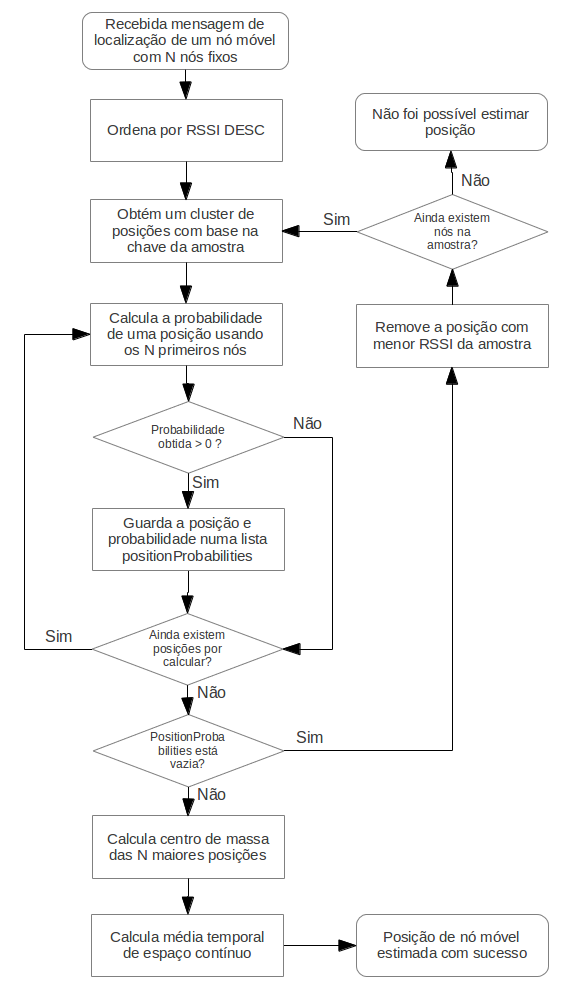
\includegraphics[width=0.85\textwidth]{img/05_horus_flow_02.png}
  \caption{Fluxograma do modo de funcionamento do n� base na localiza��o.}
  \label{fig:21:horusFlow02}
\end{figure}

\clearpage

\section{Mobilidade}
\label{chap:5:sec:5}

Neste trabalho s�o usados dois modelos de mobilidade implementados no \acs{MiXiM}. S�o eles o \textit{TurtleMobility} e o \textit{TractorMobility}. 

O \textit{TurtleMobility} permite criar um percurso com comandos introduzidos na simula��o atrav�s dum ficheiro XML. Desta forma � simulado o movimento de uma pessoa dentro de uma casa de forma simples, flex�vel e sem ter de efectuar uma compila��o do programa de cada vez que s�o feitas altera��es ao movimento. Esta op��o permite ainda que outra aplica��o possa gerar um ficheiro XML com dados reais substituindo o ficheiro existente. No Anexo \ref{list:a1:xmlTurtleMobility} est� um exemplo de um ficheiro XML de configura��o do \textit{TurtleMobility}.

Por sua vez o \textit{TractorMobility} usado especificamente para a cria��o do mapa de r�dio da simula��o, na fase \textit{offline}, permite criar de forma simples um percurso para a obten��o de pontos igualmente espa�ados, criando uma malha sobre todo o ambiente de simula��o. Na Figura \ref{fig:22:tractorMobility} � poss�vel observar um exemplo do percurso disponibilizado neste modelo. De notar que numa situa��o real seria imposs�vel construir um mapa r�dio igual devido � exist�ncia de paredes a meio do percurso, mas para um cen�rio de simula��o onde o objectivo � obter um mapa de r�dio minimamente de forma din�mica e r�pida, a solu��o encontrada � perfeitamente aceit�vel.

\begin{figure}[!htb]
  \centering
  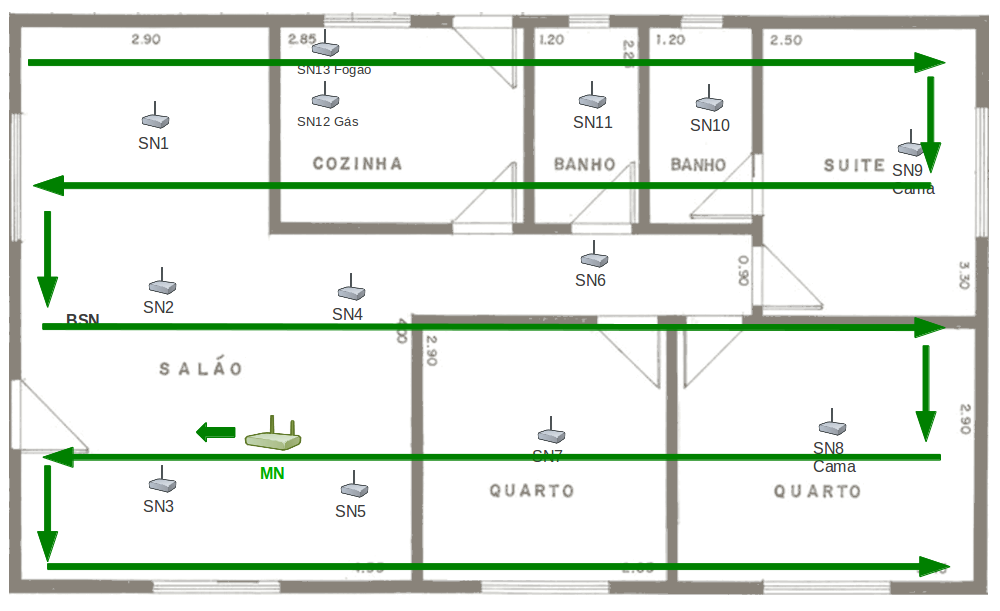
\includegraphics[width=0.85\textwidth]{img/05_tractor_mobility.png}
  \caption{Movimento do n� m�vel durante a fase \textit{offline} usando o modelo \textit{TractorMobility} dispon�vel no MiXiM.}
  \label{fig:22:tractorMobility}
\end{figure}

% Ensure that the next chapter starts in a odd page
\cleardoublepage

% %%%%%%%%%%%%%%%%%%%%%%%%%%%%%%%%%%%%%%%%%%%%%%%%%%%%%%%%%%%%%%%%%%%%%%
% State of the art
% %%%%%%%%%%%%%%%%%%%%%%%%%%%%%%%%%%%%%%%%%%%%%%%%%%%%%%%%%%%%%%%%%%%%%%

\fancychapter{Resultados}
\label{chap:6}

\section{Par�metros de Configura��o}
\label{chap:6:sec:1}

\section{Caso de Estudo 1}
\label{chap:6:sec:2}



% Ensure that the next chapter starts in a odd page
\cleardoublepage

% %%%%%%%%%%%%%%%%%%%%%%%%%%%%%%%%%%%%%%%%%%%%%%%%%%%%%%%%%%%%%%%%%%%%%%
% Conclusions
% %%%%%%%%%%%%%%%%%%%%%%%%%%%%%%%%%%%%%%%%%%%%%%%%%%%%%%%%%%%%%%%%%%%%%%

\fancychapter{Conclus�es e Trabalho Futuro}
\label{chap:7}

Com o intuito de obter uma simula��o o mais fidedigna poss�vel, foi necess�rio ao longo deste trabalho, encontrar solu��es que n�o se limitassem a simular um ou outro aspecto do problema, mas sim o conjunto completo, de funcionalidades do sistema proposto. 

Grande parte do problema ficou resolvido com o \acs{MiXiM}, no entanto foi necess�rio encontrar um protocolo de encaminhamento adequado e um sistema de localiza��o que conjuntamente, permitissem criar um sistema completamente funcional de monitoriza��o.

Este trabalho permitiu assim desenvolver uma solu��o simulada de um sistema de monitoriza��o de pessoas idosas, sem deixar de referenciar o hardware necess�rio e adquirir um conhecimento alargado do protocolo de encaminhamento \acs{AODV} e do sistema de localiza��o HORUS.

Futuramente poder� ser melhorado o protocolo de localiza��o para que deixe de ser necess�rio existir uma fase \textit{offline}, utilizando-se n�s fixos que saibam a sua pr�pria localiza��o e que com isso criem de forma autom�tica e peri�dica novos mapas r�dio sem a necessidade de interven��o.

Outra possibilidade interessante, seria implementar no n� m�vel um conjunto de camadas paralelo com r�dio bluetooth, ligando assim esse n� tamb�m a uma rede \acs{BSN} simulada, o que permitiria recriar no ambiente de trabalho eventos humanos que despoletassem mensagens, como aumento da temperatura ou batimento card�aco.

A melhoramento do modelo de obst�culos ou at� mesmo a utiliza��o de n�s reais que permitissem chegar aos par�metros do modelo utilizado, seria tamb�m uma possibilidade interessante de trabalho futuro.

% Ensure that the next chapter starts in a odd page
\cleardoublepage

% Add the Bibliography to the PDF table of contents (not the document table of contents)
\pdfbookmark[0]{Bibliografia}{bib}
% The bibliography style sheet
% \bibliographystyle{plain}
\bibliographystyle{IEEEtran}
% \bibliographystyle{apalike}
% \bibliographystyle{unsorted}
% The BiBTeX file
\bibliography{3_referencias-anexos/referencias}
\cleardoublepage

\appendix

% %%%%%%%%%%%%%%%%%%%%%%%%%%%%%%%%%%%%%%%%%%%%%%%%%%%%%%%%%%%%%%%%%%%%%%
% First appendix
% %%%%%%%%%%%%%%%%%%%%%%%%%%%%%%%%%%%%%%%%%%%%%%%%%%%%%%%%%%%%%%%%%%%%%%
\fancychapter{Ap�ndice 1 - Ficheiros XML de Configura��o}
\label{annex:a}

\fancychapter{Ap�ndice 1 - Ficheiros XML de Exemplo}
\label{annexA}

%XML CONFIG radio MAP
\begin{annex-code}{Exemplo de ficheiro XML de configura��o do mapa r�dio.}{list:a1:xmlRadioMap}
<?xml version="1.0" encoding="UTF-8"?><radioMap maxPositionPDFsSize="4">
  <position x="2" y="2">
    <staticNodePDF address="1000" mean="-6.86524" stdDev="-2.39173"/>
    <staticNodePDF address="1005" mean="-19.6319" stdDev="-15.9808"/>
    <staticNodePDF address="1001" mean="-21.0037" stdDev="-19.5426"/>
    <staticNodePDF address="1006" mean="-22.8628" stdDev="-19.3251"/>
  </position>
  <position x="4" y="2">
    <staticNodePDF address="1000" mean="-8.58641" stdDev="-7.49053"/>
    <staticNodePDF address="1006" mean="-18.8375" stdDev="-16.4028"/>
    <staticNodePDF address="1005" mean="-19.2409" stdDev="-17.7517"/>
    <staticNodePDF address="1001" mean="-19.2659" stdDev="-19.1632"/>
  </position>
  <position x="3" y="2">
    <staticNodePDF address="1000" mean="31.6669" stdDev="33.1443"/>
    <staticNodePDF address="1005" mean="-22.0094" stdDev="-19.9634"/>
    <staticNodePDF address="1006" mean="-22.8608" stdDev="-21.7965"/>
    <staticNodePDF address="1001" mean="-23.1735" stdDev="-21.8065"/>
  </position>
  <position x="6" y="2">
    <staticNodePDF address="1001" mean="-10.6905" stdDev="-6.60051"/>
    <staticNodePDF address="1000" mean="-15.8409" stdDev="-15.7502"/>
    <staticNodePDF address="1006" mean="-18.4932" stdDev="-17.3782"/>
    <staticNodePDF address="1005" mean="-19.1748" stdDev="-18.4118"/>
  </position>
  <position x="5" y="2">
    <staticNodePDF address="1000" mean="-13.661" stdDev="-11.7475"/>
    <staticNodePDF address="1001" mean="-15.1687" stdDev="-13.708"/>
    <staticNodePDF address="1006" mean="-23.314" stdDev="-20.5445"/>
    <staticNodePDF address="1005" mean="-23.8983" stdDev="-22.9379"/>
  </position>
  <position x="7" y="2">
    <staticNodePDF address="1001" mean="-9.56809" stdDev="-8.91176"/>
    <staticNodePDF address="1000" mean="-16.7335" stdDev="-15.6741"/>
    <staticNodePDF address="1006" mean="-17.5364" stdDev="-15.7507"/>
    <staticNodePDF address="1002" mean="-17.5544" stdDev="-15.1108"/>
  </position>
</radioMap>
\end{annex-code}

\begin{annex-code}{Exemplo de ficheiro XML de configura��o do m�dulo \textit{TurtleMobility} do MiXiM.}{list:a1:xmlTurtleMobility}
<movement>
	<set speed="10" angle="180"/>
	<repeat n="4">
		<forward d="50"/>
		<turn angle="90"/>
    </repeat>
    <repeat>
		<set speed="uniform(10,20)"/>
        <turn angle="uniform(-30,30)"/>
        <forward t="uniform(0.1,1)"/>
    </repeat>
</movement>
\end{annex-code}

\clearpage

\begin{annex-code}{Exemplo de ficheiro XML de configura��o de \textit{clusters} de posi��es.}{list:a1:xmlRadioMapCluster}
<?xml version="1.0" encoding="UTF-8"?>
<radioMapClusters clusterKeySize="1">
  <cluster>
    <clusterKey>
      <staticNode address="1001"/>
    </clusterKey>
    <position x="6" y="2"/>
    <position x="7" y="2"/>
    <position x="8" y="2"/>
    <position x="9" y="2"/>
    <position x="10" y="2"/>
    <position x="11" y="4"/>
    <position x="10" y="4"/>
    <position x="9" y="4"/>
    <position x="8" y="4"/>
    <position x="7" y="4"/>
    <position x="6" y="4"/>
    <position x="10" y="6"/>
  </cluster>
  <cluster>
    <clusterKey>
      <staticNode address="1000"/>
    </clusterKey>
    <position x="2" y="2"/>
    <position x="3" y="2"/>
    <position x="4" y="2"/>
    <position x="5" y="2"/>
    <position x="5" y="4"/>
    <position x="4" y="4"/>
    <position x="3" y="4"/>
    <position x="2" y="4"/>
    <position x="2" y="5"/>
    <position x="2" y="6"/>
    <position x="3" y="6"/>
  </cluster>
</radioMapClusters>
\end{annex-code}

\cleardoublepage

\end{document}
